\section{Heating, Ventilating, Air Conditioning, and Refrigeration}
\label{sec:HVAC_System_Type_Heating_Fuel_Type}

\subsection{HVAC System Heating Fuel Type}

Commercial HVAC equipment can use various heating fuel types, with the most common being natural gas, electricity, propane, fuel oil, and district heating. To reflect the variability of heating fuels in the real building stock, the ComStock workflow creates probability distributions of heating fuel types per building type at the county level. These distributions are used to assign a heating fuel type to each ComStock building model during the sampling process.

The probability distributions are informed by two data sources. First, there are the CBECS 2012 microdata, which include data on heating fuel(s), building type, and census division for the surveyed buildings. This data can be used to produce probability distributions for heating fuel by building type at the census division level. However, several data sources suggest notable variation within census divisions, which indicates that increased granularity may be needed (beyond what CBECS can provide). The heating fuel type probability distributions used in ResStock---which provides data for residential buildings at the county level---were used to add granularity. However, initial comparisons showed discrepancies between the ResStock data and the CBECS data, which is likely due to inherent differences between residential and commercial buildings. This indicated that the ResStock data should not be used directly. To rectify this, the county-level ResStock data were scaled to align with the CBECS data. This preserved the county-level variation in fuel type prevalence provided by the ResStock data, while also preserving the census division totals provided by the CBECS commercial data. District heating values were not available in the ResStock data, so the per-building-type CBECS values were used for all counties in a given census division.

In some cases, filtering down to a specific region and building type in the CBECS data yields very few samples. This can lead to unreliable conclusions for a region. To mitigate this, we took a blended approach, where some fraction of the CBECS region fuel type percentage comes from the regional samples only, and some fraction comes from the national sample for the building type. If more than 15 samples exist for a given building type and region, then 100\% of the fuel type prevalence comes from that specific region. (The threshold of 15 samples was selected baced on engineering judgment to balance process reliability and regional variability.) If there are fewer than 15 samples, the number of samples divided by 15 will be the fraction used for the region, and the remainder will use the national numbers. For example, if a region has only 12 office samples, 80\% (12\//15) of the effective CBECS regional value will come from the CBECS region, and the other 20\% will come from the national CBECS value for the building type. This will cause region/building type combinations with lower sample sizes to have a stronger inheritance of the national characteristics than the regional characteristics when we lack sufficient evidence to support this level of detail.

Some commercial building HVAC systems use multiple fuel types. For example, a VAV system with a gas furnace in the air handling unit and electric resistance coils in the reheat boxes, or a gas furnace DOAS with variable refrigerant flow (VRF) heat pumps serving the zones. This can complicate the categorization of these systems into a single primary fuel type. To address this, we determine the primary heating fuel type for the mixed fuel systems. The primary heating fuel is the heating fuel expected to carry the majority of the heating load. For example, the previously mentioned example of a VAV system with gas heat at the air handler and electric reheat would be classified as an electric-heated system, since the majority of heating for multizone VAV systems usually comes from the reheat. A full list of ComStock HVAC systems and their fuel type categories are shown in Table~\ref{tab:hvac_system_heating_fuel_categories}. Further detail on model HVAC system assignment methodology can be found in Section~\ref{sec:HVAC_System_Type}.

Figure~\ref{fig:fuel_cbecs_v_cstock} compares the prevalence of heating fuel type by stock floor area for CBECS 2012 and ComStock, by building type. In most cases, ComStock closely aligns to the CBECS 2012 values. However, there are some differences between the two sources due to randomness in the sampling process and from the use of other data sources to achieve county-level granularity in fuel type prevalence. The largest difference is in small hotels where ComStock shows 87\% of the floor area using electric heating while CBECS suggest 74\%, an absolute difference of 12\%.

\begin{figure}
  \centering
  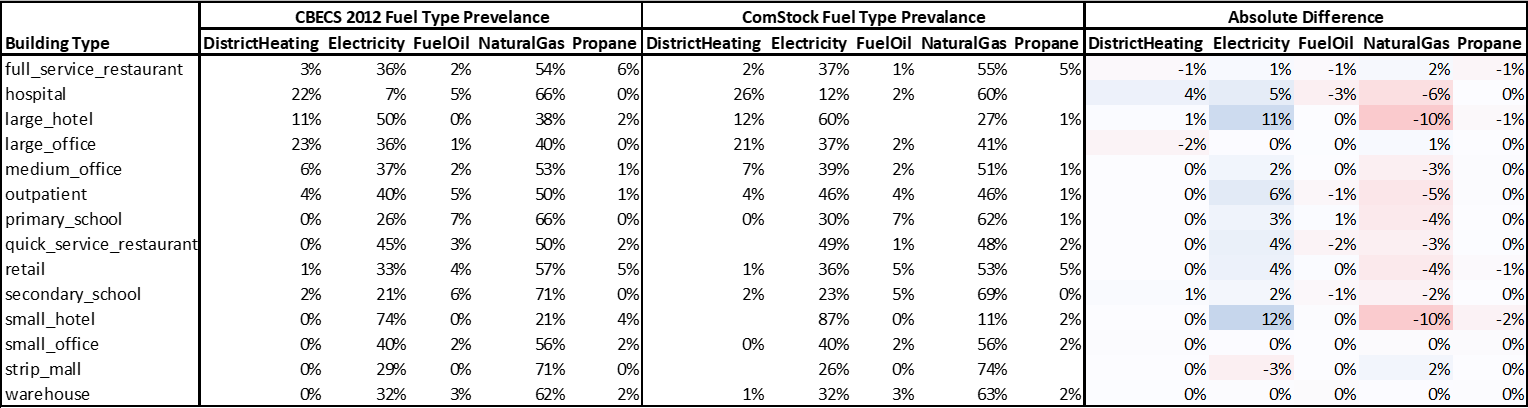
\includegraphics[width=1.10\textwidth]{figures/cbecs_comstock_fuel_type_comparison.png}
  \caption[Comparison of heating fuel type prevalence by floor area between CBECS 2012 and ComStock.]{Comparison of heating fuel type prevalence by floor area between CBECS 2012 and ComStock.}
  \label{fig:fuel_cbecs_v_cstock}
\end{figure}

The county-level prevalences of different heating fuel types are shown in Figure~\ref{fig:map_naturalgas} (natural gas), Figure~\ref{fig:map_electricity} (electricity), Figure~\ref{fig:map_fueloil} (fuel oil), Figure~\ref{fig:map_propane} (propane), and Figure~\ref{fig:map_district} (district heating).

\begin{figure}
  \centering
  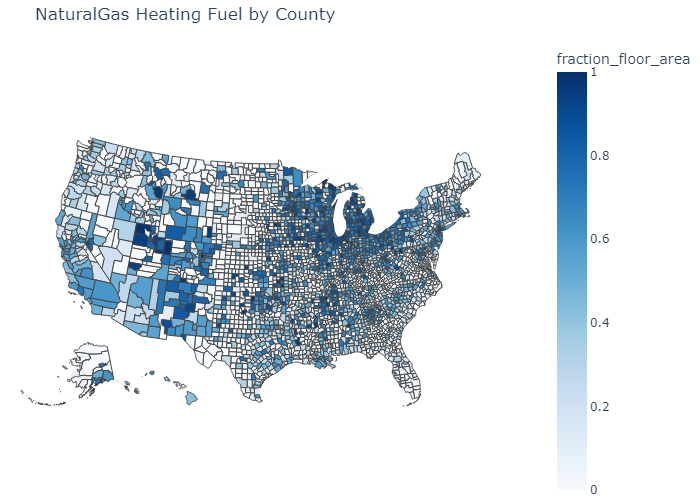
\includegraphics[width=0.8\textwidth]{figures/map_naturalgas.png}
  \caption[Fraction of ComStock models using natural gas heating/water heating per county]{Fraction of ComStock models using natural gas heating per county.}
  \label{fig:map_naturalgas}
\end{figure}

\begin{figure}
  \centering
  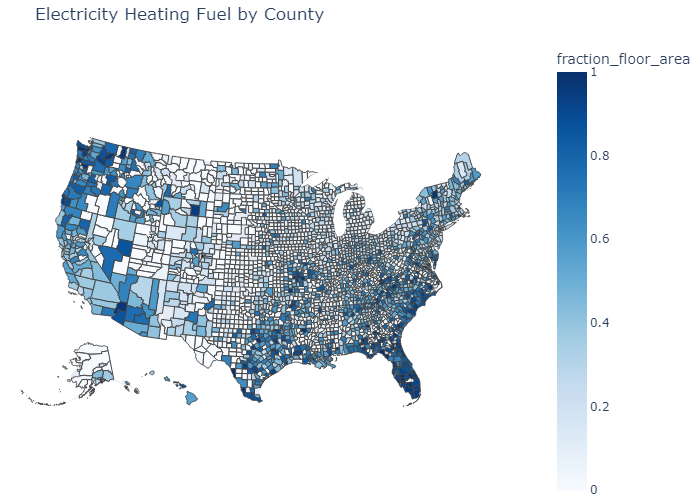
\includegraphics[width=0.8\textwidth]{figures/map_electricity.png}
  \caption[Fraction of ComStock models using electric heating/water heating per county]{Fraction of ComStock models using electric heating per county.}
  \label{fig:map_electricity}
\end{figure}

\begin{figure}
  \centering
  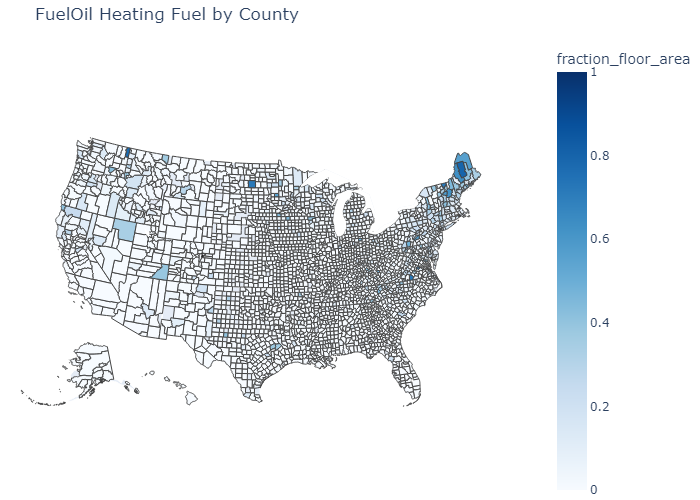
\includegraphics[width=0.8\textwidth]{figures/map_fueloil.png}
  \caption[Fraction of ComStock models using fuel oil heating/water heating per county]{Fraction of ComStock models using fuel oil heating per county.}
  \label{fig:map_fueloil}
\end{figure}

\begin{figure}
  \centering
  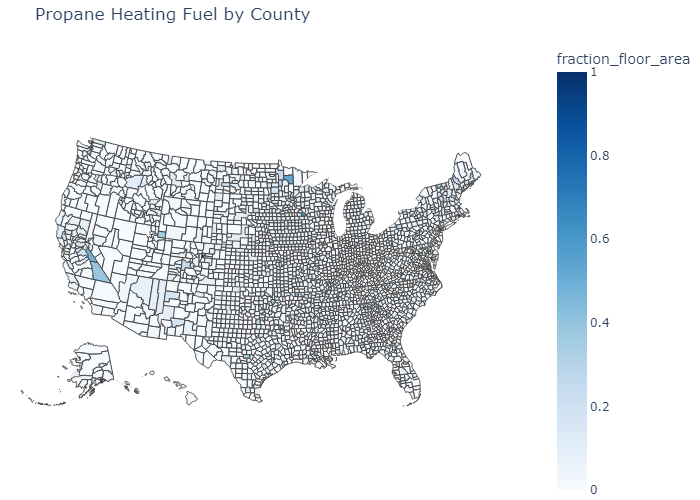
\includegraphics[width=0.8\textwidth]{figures/map_propane.png}
  \caption[Fraction of ComStock models using propane heating/water heating per county]{Fraction of ComStock models using propane heating per county.}
  \label{fig:map_propane}
\end{figure}

\begin{figure}
  \centering
  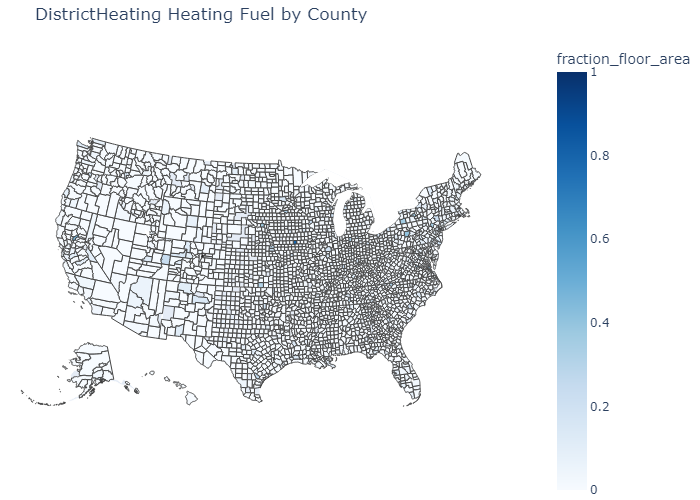
\includegraphics[width=0.8\textwidth]{figures/map_districtheating.png}
  \caption[Fraction of ComStock models using district heating/water heating per county]{Fraction of ComStock models using district heating per county.}
  \label{fig:map_district}
\end{figure}   



%figures moved to appendix

\vspace{5mm}
\subsection{HVAC System Types Probability Distributions}
\label{sec:HVAC_System_Type}

Each ComStock model is assigned a comprehensive HVAC system type. The full list of ComStock HVAC system types is shown in Table~\ref{tab:hvac_system_heating_fuel_categories}. HVAC system types are assigned to ComStock models through sampling informed by representative probability distributions. These probability distributions depend on building type, census division, and heating fuel type. For example, the distributions provide the fraction of gas-heated retail buildings in the West North Central Census Division that use each HVAC system type from Table~\ref{tab:hvac_system_heating_fuel_categories}. The probability distributions are derived from CBECS 2012 microdata, which include data on building type, census division, heating fuel type, and HVAC system type.

\begin{table}[hb!]
\small
\centering
\caption[Fuel Type Category for ComStock HVAC System Types]{Fuel Type Category for ComStock HVAC System Types}
\label{tab:hvac_system_heating_fuel_categories}
\begin{tabular}{|l|l|}
\hline
\textbf{HVAC System Type}                                   & \textbf{Heating Fuel Category} \\ \hline
Packaged variable air volume (PVAV) with gas heat with electric reheat                     & Electricity                           \\ \hline
DOAS with fan coil district chilled water with district hot water & District\_Heating        \\ \hline
Variable air volume (VAV) district chilled water with district hot water reheat         & District\_Heating        \\ \hline
PSZ-AC with gas coil                                        & Fuel                           \\ \hline
VAV chiller with PFP boxes                                  & Electricity                    \\ \hline
VAV chiller with gas boiler reheat                          & Fuel                           \\ \hline
VAV air-cooled chiller with gas boiler reheat               & Fuel                           \\ \hline
Packaged terminal air conditioner (PTAC) with electric coil                                     & Electricity                    \\ \hline
PSZ-AC with gas boiler                                      & Fuel                           \\ \hline
VAV air-cooled chiller with district hot water reheat       & District\_Heating              \\ \hline
Residential AC with residential forced air furnace          & Fuel                           \\ \hline
PSZ-AC with electric coil                                   & Electricity                    \\ \hline
VAV air-cooled chiller with parallel fan-powered (PFP) boxes                       & Electricity                    \\ \hline
Packaged terminal heat pump (PTHP)                                                        & Electricity                    \\ \hline
PVAV with gas boiler reheat                                 & Fuel                           \\ \hline
PVAV with PFP boxes                                         & Electricity                    \\ \hline
VAV chiller with district hot water reheat                  & District\_Heating              \\ \hline
DOAS with fan coil air-cooled chiller with boiler           & Fuel                           \\ \hline
DOAS with fan coil chiller with boiler                      & Fuel                           \\ \hline
DOAS with variable refrigerant flow (VRF)                                               & Electricity                    \\ \hline
Residential forced air furnace                              & Fuel                           \\ \hline
DOAS with water source heat pumps with ground source heat pump    & Electricity              \\ \hline
DOAS with water source heat pumps cooling tower with boiler & Electricity                    \\ \hline
Direct evap coolers with forced air furnace                 & Fuel                           \\ \hline
VAV district chilled water with PFP boxes                   & Electricity                    \\ \hline
PVAV with district hot water reheat                         & District\_Heating              \\ \hline
DOAS with fan coil chiller with district hot water          & District\_Heating              \\ \hline
Direct evap coolers with baseboard gas boiler               & Fuel                           \\ \hline
PTAC with gas boiler                                        & Fuel                           \\ \hline
Packaged single-zone air conditioner (PSZ-AC) with district hot water                              & District\_Heating              \\ \hline
Packaged single-zone heat pump (PSZ-HP)                                                      & Electricity                    \\ \hline
Gas unit heaters                                            & Fuel                           \\ \hline
DOAS with fan coil chiller with baseboard electric          & Electricity                    \\ \hline
PSZ-AC district chilled water with district hot water       & District\_Heating              \\ \hline
Direct evap coolers with baseboard electric                 & Electricity                    \\ \hline
VAV district chilled water with gas boiler reheat           & Fuel                           \\ \hline
Baseboard electric                                          & Electricity                    \\ \hline
DOAS with fan coil air-cooled chiller with district hot water     & District\_Heating        \\ \hline
PSZ-AC district chilled water with electric coil            & Electricity                    \\ \hline
DOAS with fan coil district chilled water with boiler       & Fuel                           \\ \hline
PTAC with gas coil                                          & Fuel                           \\ \hline
DOAS with fan coil district chilled water with baseboard electric & Electricity              \\ \hline
Baseboard gas boiler                                        & Fuel                           \\ \hline
PTAC with baseboard district hot water                      & District\_Heating              \\ \hline
DOAS with fan coil air-cooled chiller with baseboard electric     & Electricity       \\ \hline
\end{tabular}
\end{table}

\subsubsection{CBECS 2012 HVAC System Type Analysis}

To derive probability distributions of HVAC system types from the CBECS 2012 data, we first assigned one of the comprehensive ComStock HVAC system types shown in Table~\ref{tab:hvac_system_heating_fuel_categories} to the CBECS 2012 microdata samples. CBECS 2012 does not have a single survey question for the primary HVAC system type of the building, which made this analysis nontrivial. Instead, CBECS contains dozens of questions regarding the presence of several HVAC system components, fuel types, and technologies. Therefore, it is difficult to derive a deterministic HVAC system type for the CBECS 2012 building samples. Interpretation of the numerous HVAC characteristics into a complete HVAC system type needed for energy modeling involves user discretion and judgment.

In several cases, the combinations of survey responses related to the HVAC system were questionable, incomplete, or conflicting based on engineering judgment. This could be due to the survey respondent lacking information about the nuances of the building's HVAC system, the survey respondent skipping relevant questions, or the building having multiple system types, perhaps due to various activities in the building or retrofits and expansions over time. Any of these issues could create a combination of equipment for a CBECS sample that would be difficult to translate into a single, comprehensive HVAC system type without firsthand knowledge of the building. Thus, reliably discerning an HVAC system type from the survey questions can be challenging for some of the CBECS samples and requires some degree of assumption.

Based on survey responses, some CBECS samples appear to utilize multiple types of HVAC systems. For example, one sample responded affirmatively to having a chiller, packaged terminal air conditioners (PTACs), heat pumps, and a swamp cooler. However, there is no indication as to the fraction of the building serving each system type in the survey. Additionally, ComStock is not trying to model buildings with several HVAC system types. To address this, we needed to determine prioritization rules when multiple system types for a single CBECS sample appeared to be prevalent. To achieve this, we grouped systems into the following four categories: VAVs, single-zone RTU, DOAS with zone terminal units (e.g., DOAS with heat pumps, VRF), and miscellaneous single-zone equipment.

There were several cases where the assigned HVAC system for a CBECS sample was unlikely given the size and type of the building. For example, only a small percentage of small office buildings would be expected to use large, multi-zone VAV systems. Similarly, only a small percentage of very large office buildings would be expected to use single-zone RTUs or zone terminal equipment with no DOAS. To address this, we recategorized some system type assignments based on the building type and size to ensure that the resulting probability distributions were realistic.

Overall, we produced 603 probability distributions from the CBECS HVAC analysis, with dependencies based on building type, census division, and heating fuel type. These distributions are used with the ComStock sampling process, described in Section \ref{chap:3_sampling}, which ensures that HVAC system types are applied to the correct proportion of models. The prevalence of each HVAC system type in ComStock for all building types is shown in Figure~\ref{fig:hvac_sys_type_prevalence} through Figure~\ref{fig:hvac_sys_type_prevalence_warehouse}.

% AP Decided not to show this table as the information is conveyed more usefully in the figures below
% \begin{center}
\begin{longtable}{|p{5cm}|p{1.5cm}|p{1.5cm}|p{1.5cm}|p{1.5cm}|p{1.5cm}|p{1.5cm}|p{1.5cm}|p{1.5cm}|p{1.5cm}|p{1.5cm}|p{1.5cm}|p{1.5cm}|p{1.5cm}|p{1.5cm}|}
\caption[HVAC System Type Prevalence]{HVAC System Type Prevalence by Building Type} \\ \hline
\label{tab:hvac_system_types}
\textbf{ComStock System Type} &
  \textbf{full service restaurant} &
  \textbf{hospital} &
  \textbf{large hotel} &
  \textbf{large office} &
  \textbf{medium office} &
  \textbf{outpatient} &
  \textbf{primary school} &
  \textbf{quick service restaurant} &
  \textbf{retail} &
  \textbf{secondary school} &
  \textbf{small hotel} &
  \textbf{small office} &
  \textbf{strip mall} &
  \textbf{warehouse} \\ \hline
\endfirsthead
\multicolumn{2}{c} {{\bfseries \tablename \thetable{} -- continued from previous page}} \\ \hline
\textbf{ComStock System Type} &
  \textbf{full service restaurant} &
  \textbf{hospital} &
  \textbf{large hotel} &
  \textbf{large office} &
  \textbf{medium office} &
  \textbf{outpatient} &
  \textbf{primary school} &
  \textbf{quick service restaurant} &
  \textbf{retail} &
  \textbf{secondary school} &
  \textbf{small hotel} &
  \textbf{small office} &
  \textbf{strip mall} &
  \textbf{warehouse} \\ \hline
\endhead
\small
Baseboard electric                                                & 0    & 0    & 0    & 0    & 0    & 0    & 0    & 0    & 0.5  & 0    & 0    & 0    & 0    & 0.6  \\ \hline
Baseboard gas boiler                                              & 0    & 0    & 0    & 0    & 0    & 0    & 0    & 0    & 0    & 0    & 0    & 0    & 0    & 0    \\ \hline
DOAS with VRF                                                     & 0    & 0    & 0.4  & 0.8  & 1.7  & 1.3  & 0.3  & 0    & 0    & 0    & 0    & 1.5  & 0    & 0.3  \\ \hline
DOAS with fan coil air-cooled chiller with baseboard electric     & 0    & 0    & 0.1  & 0    & 0    & 0    & 0    & 0    & 0    & 0    & 0    & 0    & 0    & 0    \\ \hline
DOAS with fan coil air-cooled chiller with boiler                 & 0    & 0.2  & 2.7  & 0.3  & 0    & 0.5  & 0.9  & 0    & 0    & 1.9  & 0    & 0    & 0    & 0    \\ \hline
DOAS with fan coil air-cooled chiller with district hot water     & 0    & 0.1  & 0    & 1.1  & 0    & 0    & 0    & 0    & 0    & 0    & 0    & 0    & 0    & 0    \\ \hline
DOAS with fan coil chiller with baseboard electric                & 0    & 0    & 0.6  & 0.1  & 0    & 0    & 0    & 0    & 0    & 0    & 0    & 0    & 0    & 0    \\ \hline
DOAS with fan coil chiller with boiler                            & 0    & 0.5  & 6.2  & 0.4  & 2.8  & 0    & 0.2  & 0    & 0    & 0.5  & 0.8  & 0.4  & 0    & 0    \\ \hline
DOAS with fan coil chiller with district hot water                & 0    & 0    & 1.3  & 0    & 0    & 0    & 0    & 0    & 0    & 0    & 0    & 0    & 0    & 0    \\ \hline
DOAS with fan coil district chilled water with baseboard electric & 0    & 0    & 0.1  & 0    & 0    & 0    & 0    & 0    & 0    & 1.6  & 0    & 0    & 0    & 0    \\ \hline
DOAS with fan coil district chilled water with boiler             & 0    & 0    & 1.8  & 0    & 0    & 0    & 0    & 0    & 0    & 0    & 0    & 0    & 0    & 0    \\ \hline
DOAS with fan coil district chilled water with district hot water & 0.1  & 0    & 0.5  & 0.1  & 0.1  & 0    & 0    & 0    & 0    & 0.2  & 0    & 0    & 0    & 0    \\ \hline
DOAS with water source heat pumps cooling tower with boiler       & 0    & 0.7  & 8    & 5.3  & 1.8  & 0.4  & 3.1  & 0    & 0    & 3.1  & 3    & 0.3  & 0.1  & 0    \\ \hline
DOAS with water source heat pumps with ground source heat pump    & 0    & 0    & 6.3  & 1.1  & 0    & 0.6  & 2.1  & 0    & 0    & 4.8  & 0    & 1.2  & 0    & 0    \\ \hline
Direct evap coolers with baseboard electric                       & 0.5  & 0    & 0    & 0    & 0    & 0    & 0    & 0    & 0.6  & 0    & 0    & 0    & 0.6  & 0    \\ \hline
Direct evap coolers with baseboard gas boiler                     & 0    & 0    & 0    & 0    & 0    & 1.2  & 0.4  & 0    & 0    & 0    & 0    & 0    & 0    & 0    \\ \hline
Direct evap coolers with forced air furnace                       & 0.9  & 0    & 0    & 0    & 0.8  & 0    & 0    & 1.3  & 1.6  & 1.4  & 0    & 0.3  & 0.6  & 0.5  \\ \hline
Gas unit heaters                                                  & 0.5  & 0    & 0    & 0    & 0    & 0    & 0    & 0    & 0    & 0    & 0    & 0.3  & 0    & 2.7  \\ \hline
PSZ-AC district chilled water with district hot water             & 0.6  & 0    & 0    & 0    & 0.5  & 0    & 0    & 0    & 0    & 1.3  & 0    & 0    & 0    & 0    \\ \hline
PSZ-AC district chilled water with electric coil                  & 0    & 0    & 0    & 0    & 0    & 0    & 4    & 0    & 0    & 5.9  & 0    & 0.4  & 0    & 0    \\ \hline
PSZ-AC with district hot water                                    & 0    & 0    & 0    & 0.3  & 1.3  & 0.3  & 0.2  & 0    & 0.5  & 0.6  & 0    & 0    & 0    & 0.1  \\ \hline
PSZ-AC with electric coil                                         & 25.4 & 4.3  & 0    & 3.3  & 15.7 & 22.4 & 16.6 & 44.1 & 19.4 & 11.5 & 0    & 24.6 & 32.3 & 27.2 \\ \hline
PSZ-AC with gas boiler                                            & 3.1  & 6.4  & 0    & 3.3  & 9.1  & 4.3  & 9.4  & 2.7  & 1.5  & 4.7  & 0    & 3    & 0.2  & 1.5  \\ \hline
PSZ-AC with gas coil                                              & 47.2 & 0    & 0    & 3.5  & 15.2 & 39.6 & 23.1 & 41.6 & 41   & 6.6  & 0    & 40.3 & 46.3 & 36.2 \\ \hline
PSZ-HP                                                            & 0    & 0    & 0    & 0    & 1.5  & 0.2  & 0    & 0    & 0    & 0    & 0    & 0    & 2.6  & 0    \\ \hline
PTAC with baseboard district hot water                            & 0    & 0.1  & 0    & 0    & 0    & 0    & 0    & 0    & 0    & 0    & 0    & 0    & 0    & 0    \\ \hline
PTAC with electric coil                                           & 0.9  & 2.9  & 30.9 & 0    & 0.3  & 3.8  & 0.4  & 1.8  & 1    & 0    & 27.5 & 2.6  & 1.1  & 0.7  \\ \hline
PTAC with gas boiler                                              & 0    & 0    & 0    & 0    & 0    & 0    & 0    & 0    & 0    & 0    & 5.8  & 0    & 0    & 0    \\ \hline
PTAC with gas coil                                                & 0    & 0    & 0.6  & 0    & 0    & 0    & 0    & 0    & 0.6  & 0    & 0    & 0.6  & 0.6  & 0    \\ \hline
PTHP                                                              & 0    & 0    & 27.6 & 0    & 0    & 0    & 0    & 4.5  & 13.2 & 10.1 & 43.2 & 12.3 & 2.2  & 9.1  \\ \hline
PVAV with PFP boxes                                               & 1    & 0.1  & 0    & 7.6  & 6.2  & 6.1  & 5.8  & 0    & 1.7  & 1.9  & 0    & 1.1  & 2    & 1.4  \\ \hline
PVAV with district hot water reheat                               & 0    & 2.9  & 0    & 4.7  & 0.2  & 0    & 0    & 0    & 0    & 0    & 0    & 0    & 0    & 0    \\ \hline
PVAV with gas boiler reheat                                       & 1.6  & 3    & 0    & 9.5  & 12.3 & 3.9  & 9.1  & 0    & 2.6  & 5.8  & 0    & 0.7  & 1.6  & 1.4  \\ \hline
PVAV with gas heat with electric reheat                           & 0.5  & 1.7  & 0    & 5.3  & 11   & 2.1  & 4.4  & 0    & 1.7  & 3.8  & 0    & 1.9  & 8    & 2.6  \\ \hline
Residential AC with residential forced air furnace                & 16.8 & 0    & 13.1 & 0.3  & 4.8  & 7    & 8.7  & 2.9  & 12   & 8.9  & 17.6 & 8.1  & 1.4  & 8.9  \\ \hline
Residential forced air furnace                                    & 0    & 0    & 0    & 0    & 0    & 0    & 0.1  & 1.1  & 1.9  & 4.7  & 2    & 0.1  & 0    & 6.6  \\ \hline
VAV air-cooled chiller with PFP boxes                             & 0.5  & 0.3  & 0    & 1.8  & 0.1  & 1.5  & 1.5  & 0    & 0    & 0.9  & 0    & 0    & 0    & 0    \\ \hline
VAV air-cooled chiller with district hot water reheat             & 0    & 3.3  & 0    & 0.3  & 0.9  & 0.1  & 0    & 0    & 0    & 0    & 0    & 0    & 0    & 0    \\ \hline
VAV air-cooled chiller with gas boiler reheat                     & 0    & 25.3 & 0    & 4.5  & 4.4  & 0.9  & 5.4  & 0    & 0    & 13.1 & 0    & 0    & 0    & 0.1  \\ \hline
VAV chiller with PFP boxes                                        & 0    & 3.4  & 0    & 11.4 & 3.1  & 1.9  & 0    & 0    & 0    & 0.2  & 0    & 0    & 0.5  & 0    \\ \hline
VAV chiller with district hot water reheat                        & 0    & 1.9  & 0    & 5.3  & 0    & 0.2  & 0    & 0    & 0    & 0    & 0    & 0    & 0    & 0    \\ \hline
VAV chiller with gas boiler reheat                                & 0    & 35.2 & 0    & 19.1 & 2.7  & 1.1  & 3.7  & 0    & 0    & 5.4  & 0    & 0.2  & 0    & 0.1  \\ \hline
VAV district chilled water with PFP boxes                         & 0.3  & 0    & 0    & 0    & 1.1  & 0    & 0.7  & 0    & 0    & 0.7  & 0    & 0    & 0    & 0    \\ \hline
VAV district chilled water with district hot water reheat         & 0.2  & 7.7  & 0    & 10   & 2.5  & 0.1  & 0    & 0    & 0    & 0.2  & 0    & 0.1  & 0    & 0    \\ \hline
VAV district chilled water with gas boiler reheat                 & 0    & 0.3  & 0    & 0.3  & 0.1  & 0.8  & 0    & 0    & 0    & 0    & 0    & 0    & 0    & 0    \\ \hline
\end{longtable}
\end{center} % TODO Format table: This may just be too big with the long names
%figures in appendix

\subsection{HVAC System Sizing}

HVAC systems in ComStock are sized using standard EnergyPlus sizing routines. The program uses design day information from the respective weather file coupled with the model's specific control settings and performs sizing runs to determine equipment capacity sizing. Per ASHRAE 90.1 Appendix G, systems are oversized by 15\% for cooling and 25\% for heating. Note that sizing results for a model will be impacted by several control properties specific to the model, such as supply air temperature control, thermostat set points, and outdoor ventilation rates, which are described in later sections.

\subsection{Outdoor Air Ventilation Rates}

Commercial buildings require outdoor ventilation air when the building is occupied. The design outdoor air rate for a system is the minimum amount of outdoor air the system must supply while the building is occupied. The amount of outdoor air required for an HVAC system is calculated by the combined needs of the space type(s) served by a system.

ComStock design outdoor air ventilation rates follow the requirements set forth by ASHRAE Standard 62.1: Ventilation for Acceptable Indoor Air Quality (non-California models), or by DEER (California models). Both of these sources dictate the minimum design outdoor air flow rate by space type. The minimum outdoor air requirements for each space type are composed of a flow rate per person, a flow rate per area, and in some cases, an exhaust rate. Combined, these components determine the design outdoor air requirement for each space and its respective HVAC system. Table~\ref{tab:outdoor_air_table} and Table~\ref{tab:outdoor_air_table_deer} show the average design outdoor air flow rate per area (cfm/m\textsuperscript{2}) for non-California models and California models, respectively. These averages are influenced by the number of buildings of each type and their vintage. Both methods are heavily influenced by the space type composition of the model; ComStock models assume space type ratios for building types, with some building types having variation in the space type ratios. ComStock space types are described further in Section~\ref{sec:space_type_ratios}.

Some ComStock HVAC system types are residential style systems (denoted ``residential'' in Table~\ref{tab:hvac_system_heating_fuel_categories}). These systems do not include ventilation air and are an exception to the aforementioned ASHRAE-62.1 outdoor air methodology. Although commercial buildings all require outdoor ventilation air per code, some commercial buildings in the stock use residential systems without outdoor air. This is reflected in ComStock through the use of these residential system types. ComStock's HVAC system selection methodology is described further in Section~\ref{sec:HVAC_System_Type}.

\begin{table}
\small
\centering
\caption[Design Outdoor Air Rates---Outside California]{Design Outdoor Air Rates by Building Type and HVAC Code Template for Buildings Outside California}
\label{tab:outdoor_air_table}
\begin{tabular}{|p{2.5cm}|p{1.4cm}|p{1.4cm}|p{1.4cm}|p{1.4cm}|p{1.4cm}|p{1.4cm}|}
\hline
\textbf{Building   Type} &
  \textbf{Pre-1980 (cfm/sf)} &
  \textbf{1980--2004   (cfm/sf)} &
  \textbf{90.1-2004 (cfm/sf)} &
  \textbf{90.1-2007 (cfm/sf)} &
  \textbf{90.1-2010 (cfm/sf)} &
  \textbf{90.1-2013 (cfm/sf)} \\ \hline
\textbf{FullService\-Restaurant}  & 1.103 & 1.103 & 1.107 & 1.048 & 1.067 & 1.077 \\ \hline
\textbf{Grocery}                 & 0.225     & 0.225 & 0.225 & 0.175 & 0.175 & 0.175 \\ \hline
\textbf{Hospital}                 & -     & 0.258 & 0.254 & 0.258 & 0.258 & 0.258 \\ \hline
\textbf{LargeHotel}               & 0.240 & 0.240 & 0.240 & 0.224 & 0.234 & 0.226 \\ \hline
\textbf{LargeOffice}              & 0.098 & 0.098 & 0.098 & 0.098 & 0.098 & 0.098 \\ \hline
\textbf{MediumOffice}             & 0.100 & 0.100 & 0.100 & 0.098 & 0.098 & 0.098 \\ \hline
\textbf{Outpatient}               & 0.215 & 0.215 & 0.223 & 0.215 & 0.215 & 0.215 \\ \hline
\textbf{PrimarySchool}            & 0.376 & 0.376 & 0.378 & 0.374 & 0.374 & 0.374 \\ \hline
\textbf{QuickService\-Restaurant} & 0.935 & 0.935 & 0.935 & 0.849 & 0.884 & 0.886 \\ \hline
\textbf{RetailStandalone}         & 0.276 & 0.276 & 0.276 & 0.268 & 0.270 & 0.270 \\ \hline
\textbf{RetailStripmall}          & 0.449 & 0.461 & 0.461 & 0.449 & 0.451 & 0.453 \\ \hline
\textbf{SecondarySchool}          & 0.547 & 0.547 & 0.547 & 0.543 & 0.542 & 0.542 \\ \hline
\textbf{SmallHotel}               & -     & -     & 0.138 & 0.100 & 0.100 & 0.100 \\ \hline
\textbf{SmallOffice}              & 0.100 & 0.100 & 0.100 & 0.100 & 0.098 & 0.098 \\ \hline
\textbf{Warehouse}                & 0.049 & 0.049 & 0.049 & 0.051 & 0.051 & 0.051 \\ \hline
\end{tabular}
\end{table}
\begin{table}
\small
\centering
\caption[Design Outdoor Air Rates---Inside California]{Design Outdoor Air Rates by Building Type and HVAC Code Template for Buildings Inside California}
\label{tab:outdoor_air_table_deer}
\begin{tabular}{|p{1in}|p{0.4in}|p{0.4in}|p{0.4in}|p{0.4in}|p{0.4in}|p{0.4in}|p{0.4in}|p{0.4in}|p{0.4in}|}
\hline
\textbf{Building   Type} &
  \textbf{DEER Pre-1975 (cfm/sf)} &
  \textbf{DEER 1985 (cfm/sf)} &
  \textbf{DEER 1996 (cfm/sf)} &
  \textbf{DEER 2003 (cfm/sf)} &
  \textbf{DEER 2007 (cfm/sf)} &
  \textbf{DEER 2011 (cfm/sf)} &
  \textbf{DEER 2014 (cfm/sf)} &
  \textbf{DEER 2015 (cfm/sf)} &
  \textbf{DEER 2017 (cfm/sf)} \\ \hline
\textbf{FullService\-Restaurant}  & 0.540 & 0.540 & 0.540 & 0.540 & 0.540 & 0.540 & 0.540 & 0.540 & 0.540 \\ \hline
\textbf{Hospital}                 & -     & 0.152 & 0.152 & 0.152 & 0.152 & 0.152 & 0.152 & 0.152 & -     \\ \hline
\textbf{LargeHotel}               & 0.000 & 0.104 & 0.104 & 0.104 & 0.104 & 0.104 & 0.104 & 0.104 & 0.104 \\ \hline
\textbf{LargeOffice}              & 0.108 & 0.108 & 0.108 & 0.108 & 0.108 & 0.108 & 0.108 & 0.108 & 0.108 \\ \hline
\textbf{MediumOffice}             & -     & 0.108 & 0.108 & 0.108 & 0.108 & 0.108 & 0.108 & 0.108 & 0.108 \\ \hline
\textbf{Outpatient}               & 0.108 & 0.108 & 0.108 & 0.108 & 0.108 & 0.108 & 0.108 & 0.108 & 0.108 \\ \hline
\textbf{PrimarySchool}            & -     & 0.447 & 0.447 & 0.447 & 0.447 & 0.447 & 0.447 & 0.447 & 0.447 \\ \hline
\textbf{QuickService\-Restaurant} & 0.439 & 0.439 & 0.439 & 0.439 & 0.439 & 0.439 & 0.439 & 0.439 & 0.439 \\ \hline
\textbf{RetailStandalone}         & 0.268 & 0.268 & 0.268 & 0.268 & 0.268 & 0.268 & 0.268 & 0.268 & 0.268 \\ \hline
\textbf{RetailStripmall}          & 0.327 & 0.323 & 0.323 & 0.323 & 0.323 & 0.323 & 0.325 & 0.323 & 0.323 \\ \hline
\textbf{SecondarySchool}          & 0.433 & 0.433 & 0.433 & 0.433 & 0.433 & 0.433 & 0.433 & 0.433 & 0.433 \\ \hline
\textbf{SmallHotel}               & 0.069 & 0.069 & 0.069 & 0.069 & 0.069 & 0.069 & 0.069 & 0.069 & 0.069 \\ \hline
\textbf{SmallOffice}              & 0.077 & 0.077 & 0.077 & 0.077 & 0.077 & 0.077 & 0.077 & 0.077 & 0.077 \\ \hline
\textbf{Warehouse}                & 0.150 & 0.150 & 0.150 & 0.150 & 0.150 & 0.150 & 0.150 & 0.150 & 0.150 \\ \hline
\end{tabular}
\end{table}

\pagebreak
\subsection{Fan Systems}

Fans are used in all ComStock HVAC systems except those that rely on radiant heat transfer, such as baseboards. Fans induce pressure in the air stream of HVAC equipment, producing the airflow needed for space conditioning and/or outdoor air ventilation.

\subsubsection{Fan Power}

Fan power determines the amount of energy it takes a fan system to provide a certain amount of airflow. The fan power requirements of each HVAC system are a function of the total pressure drop of the air stream that the fan system will need to overcome (e.g., from filters, coils, air ducts) as well as the efficiency of the fan blades and fan motor.

Fan power in ComStock is determined by ASHRAE-90.1 code requirements. ASHRAE-90.1 determines fan power primarily based on the system type. Constant air volume, variable air volume, and unitary zone equipment are all assigned different fan power allowances.

For implementation in ComStock, fan power is determined based on the static pressure of the air delivery system, the efficiencies of the fan/motor system, and the airflow of the system. The static pressure is based on the HVAC system type and the maximum airflow of the system, as shown in Table~\ref{tab:fan_power}. The fan motor efficiencies are a function of the motor size and HVAC code year, as shown in Table~\ref{tab:fan_motor_efficiencies}.

The addition of energy recovery ventilators (ERVs) in HVAC air loops can add additional static pressure to the air system and therefore result in a higher fan power requirement. ComStock accounts for this additional fan power in the ERV wheel power rather than the fan itself; this allows for improved accuracy during ERV bypass modes (where the airflow bypasses the additional static pressure of the ERV system). See Section~\ref{sec:erv} for more information on ComStock ERV systems.

%TODO: VAV fan curves used

% Please add the following required packages to your document preamble:
% \usepackage{multirow}
\begin{table}[h!]
\centering
\small
\caption{Fan Pressure Rise and Efficiency}
\label{tab:fan_power}
\begin{tabular}{|p{1.8cm}|p{1.8cm}|p{1.8cm}|p{1.8cm}|p{1.8cm}|p{1.8cm}|p{1.8cm}|}
\hline
\textbf{Fan Type} &
  \textbf{Max Airflow (cfm)} &
  \textbf{Pressure Rise (in. H$_2$O)} &
  \textbf{Fan Power Minimum Flow Fraction} &
  \textbf{Fan Impeller Efficiency} &
  \textbf{Motor Efficiency} &
  \textbf{Total Fan Efficiency} \\ \hline
\multirow{3}{*}{\parbox{1.8cm}{\textbf{Constant Volume and DOAS}}} &
  \textless 7,437 &
  2.5 &
  \multirow{3}{*}{1} &
  \multirow{6}{*}{0.65} &
  \multirow{9}{*}{\parbox{1.4cm}{See motor efficiency lookup table}} &
  \multirow{9}{*}{\parbox{1.4cm}{(Fan Impeller Eff.) X (Motor Eff.)}} \\ \cline{2-3}
                                                & $\ge$7,537 and \textless{}20,000 & 4.46 &                       &                       &  &  \\ \cline{2-3}
                                                & $\ge$20,000                      & 4.09 &                       &                       &  &  \\ \cline{1-4}
\multirow{3}{*}{\parbox{1.4cm}{\textbf{Variable   Air Volume}}} & \textless 4,648                            & 4    & \multirow{3}{*}{0.25} &                       &  &  \\ \cline{2-3}
                                                & $\ge$4,648 and \textless 20,000  & 6.32 &                       &                       &  &  \\ \cline{2-3}
                                                & $\ge$20,000                     & 5.58 &                       &                       &  &  \\ \cline{1-5}
\textbf{PTAC/PTHP, WSHP, VRF}                   & \textgreater{}0                            & 1.33 & 1                     & \multirow{3}{*}{0.55} &  &  \\ \cline{1-4}
\textbf{Four Pipe Fan   Coil}                   & \textgreater{}0                            & 1.09 & 1                     &                       &  &  \\ \cline{1-4}
\textbf{Unit Heater}                            & \textgreater{}0                            & 0.2  & 1                     &                       &  &  \\ \hline
\end{tabular}
\end{table}

\subsubsection{Fan Controls}

This section describes the operation of fan systems during the hours a building is occupied. Details on the operation of fan systems during unoccupied hours are described in Section~\ref{sec:unoccupied_ahu_operation}.

\paragraph{HVAC Systems Providing Outdoor Air}

As required by ASHRAE-90.1, HVAC systems in commercial buildings must constantly provide the minimum design outdoor air flow rates when the building is occupied. HVAC systems in ComStock follow this control requirement. For constant volume systems, the fan system will run continuously at design airflow during occupied hours. For VAV systems, the fan system will run continuously between the minimum and maximum airflow of the system during occupied hours, always ensuring that the total system airflow meets the airflow needs of every zone.

\paragraph{HVAC Systems Not Providing Outdoor Air}

Systems that do not directly provide outdoor air, such as zone-level unitary systems coupled with a DOAS, do not need to run fans continuously. Therefore, these systems are controlled to cycle the fan system on only when required to maintain zone thermostat set points. Otherwise, the fans are allowed to turn off. This is also the control logic for any residential-style system in ComStock that does not provide outdoor air.
% TODO: kitchen exhaust fans (if I can get to this after everything else)

\subsection{Pump Systems}

Pumps are used to induce flow in building hydronic loops. This includes heating water loops, cooling water loops, condenser water loops, and ground-source heat pump water loops.
%TODO service water pump loops

\subsubsection{Pump Power}

Pump power is a function of the pressure head of the hydronic loop and the pump efficiency. The pressure heads in ComStock hydronic systems are set to reflect the baseline requirements specified in ASHRAE-90.1, noting that each hydronic loop type has its own specifications. The pressure heads used for the various ComStock hydronic loop types are specified in Table~\ref{tab:pumps}. Primary-only pump configurations use a single hydronic loop system between the boilers/chillers and the heating/cooling coils for space conditioning. A primary-secondary system uses a primary loop for circulating water between the boilers/chillers, and a secondary loop for supplying the the plant fluid to the heating/cooling coils. Pump motor efficiencies are derived using the same motor efficiency lookup tables used for fans (Table~\ref{tab:fan_motor_efficiencies}).

\subsubsection{Pump Controls}

All pumps in ComStock are set to use intermittent controls, meaning that they can cycle off when there is no load present in the loop. Constant volume pumps are controlled to ride the pump curve, as specified by ASHRAE-90.1, whereas variable speed pumps can adjust their speed to modulate flow as needed. Variable speed pumps all have a minimum flow ratio of 0\% in ComStock. This value is likely too low and underestimates pumping energy, as most pump systems can only reduce flow as low as 30\%--50\% in order to maintain proper operation of chillers, boilers, etc. The assignment methodology for variable speed pumps is specified in Table~\ref{tab:pumps}.

\begin{table}[h!]
\centering
\small
\caption{Pump Configuration and Pressure Rise for Hydronic Loops}
\label{tab:pumps}
\begin{tabular}{|p{2.5cm}|p{2.5cm}|p{2.5cm}|p{2.5cm}|p{2.5cm}|}
\hline
\textbf{Loop Type} &
  \textbf{Pump Configuration} &
  \textbf{Primary Pump Head (ft w.c.)} &
  \textbf{Secondary Pump Head (ft w.c.)} &
  \textbf{VFD Pump?} \\ \hline
\textbf{Hot Water Loop} &
  \multirow{2}{*}{Primary-only} &
  \multirow{2}{*}{60} &
  \multirow{2}{*}{-} &
%   \multirow{2}{*}{Variable speed when building area \textgreater{}120,000sf} \\ \cline{1-1}
  \multirow{2}{*}{\parbox{2.5cm}{Variable speed when building area \textgreater{}120,000 ft$^2$}} \\
\textbf{District   Heating Loop} &
   &
   &
   &
   \\ \hline
\textbf{Water-Cooled   Chiller Loop} &
  Constant-primary,   variable-secondary &
  15 &
  45 &
  Secondary pump always variable speed \\ \hline
\textbf{Air-Cooled   Chiller Loop} &
  \multirow{2}{*}{Primary-only} &
  \multirow{2}{*}{60} &
  \multirow{2}{*}{-} &
%   \multirow{2}{*}{Variable speed when cooling capacity \textgreater{}300   tons} \\ \cline{1-1}
  \multirow{2}{*}{\parbox{2.5cm}{Variable speed when cooling capacity \textgreater{}300 tons}} \\
\textbf{District   Cooling Loop} &
   &
   &
   &
   \\ \hline
\textbf{Condenser   Water Loop} &
  Primary-only &
  50 &
  - &
  Always constant speed \\ \hline
\textbf{GSHP Condenser   Water Loop} &
  Primary-only &
  60 &
  - &
  Always constant speed \\ \hline
\end{tabular}
\end{table}

%TODO: Make sure VAV is correct
%TODO: Add performance curves for VAV pumps

\subsection{Thermostat Set Points}
Thermostat set points, both heating and cooling, dictate the target indoor temperature range for the HVAC system to satisfy. The cooling thermostat set point will set the upper temperature limit, whereas the heating thermostat set point will set the lower temperature limit.

Thermostat set points are implemented in ComStock through square-wave schedules. Each model is assigned a set point temperature, which is the temperature the HVAC system must maintain during occupied hours, and a setback temperature, which is the temperature the HVAC system must maintain during unoccupied hours (note that some models have no setback temperature). The set point and setback temperatures used in the models are described later in this section. The timing of the set point and setback temperatures align with the building occupancy schedules discussed in Section~\ref{sec:hoo}.

\subsubsection{Thermostat Set Points Informed by Building Automation System Data}
\label{section:therm_setpoints_bas}

This section outlines the ComStock thermostat set point assignment methodology for the following building types: full service restaurant, large office, medium office, primary school, quick service restaurant, retail standalone, retail strip mall, secondary school, and small office.

All ComStock building types, excluding hospitals, outpatient, warehouses, and hotels, utilize building automation system (BAS) data to inform distributions of thermostat set points. The methodology behind this approach is described in this section. The intent is to include heating and cooling thermostat set point variability between ComStock models to reflect the thermostat set point variability between real buildings. For example, some offices could be expected to set their heating thermostat to 72°F, whereas others might set it to 70°F. The ComStock methodology allows this variation to exist in the models.

Building automation data from three industry-provided private data sources with over 3,700 buildings were used to derive the distributions of thermostat set points that are used to assign set points to the applicable ComStock models. Table~\ref{tab:bas_thermostat_count_by_btype} shows the counts of buildings with thermostat data available in the data set by building type. The data set includes the time series heating and cooling set points that were used to determine the occupied heating and cooling set points for each building. In turn, these were used to create probability distributions of thermostat set points by building type when aggregating across the data set. For building types with less than 25 samples in the data set, the distribution for all building types was used, as smaller sample sizes cannot reliably be extrapolated to represent a population. The resulting heating and cooling probability distributions, per applicable building type, are shown in Figure~\ref{fig:htg_therm_setpoints} and Figure~\ref{fig:clg_therm_setpoints}, respectively. Note that some outliers exist in the data set at very low prevalence, such as offices with heating set points of 61°F. These outliers are incorporated into ComStock models at a similar low prevalence to reflect the wide diversity of commercial buildings.

\begin{table}[h!]
\small
\caption[Building Counts with Thermostat Data]{Building Counts With Thermostat Data by Building Type}
\label{tab:bas_thermostat_count_by_btype}
    \centering
    \begin{tabular}{|l|l|}
    \hline
        \textbf{Building Type} &
        \textbf{Building Count} \\ \hline
        Food Service/Restaurant & 1,817 \\ \hline
        Mercantile Retail & 1,692 \\ \hline
        Food Sales/Grocery & 164 \\ \hline
        Office & 31 \\ \hline
        School & 16 \\ \hline
        Warehouse & 4 \\ \hline
        Hotel & 4 \\ \hline
        Hospital & 2 \\ \hline
        Outpatient & 2 \\ \hline
    \end{tabular}
\end{table}

\begin{figure}
    \centering 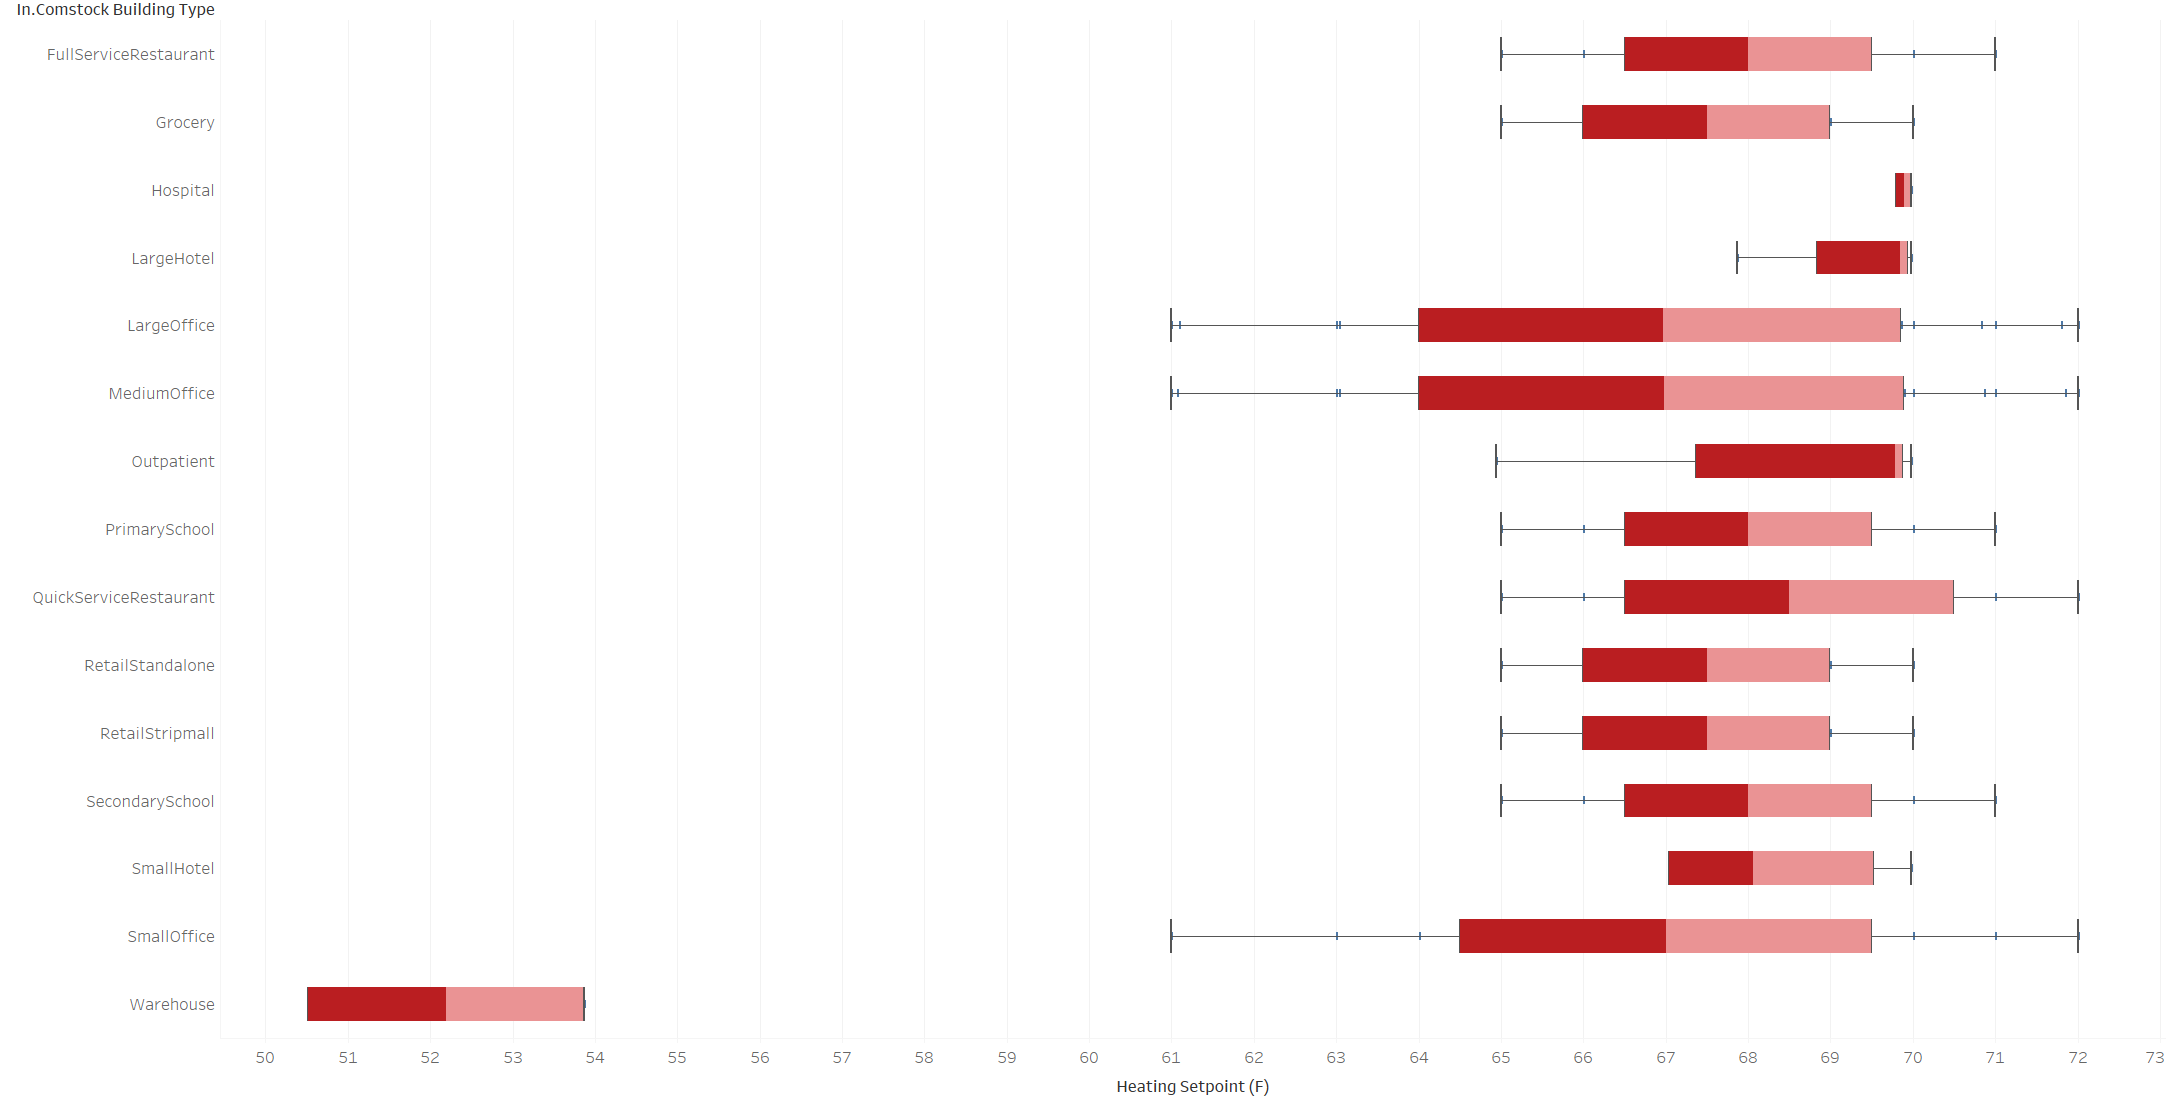
\includegraphics[width=1.0\textwidth]{figures/heating_setpoints.png}
    \caption{Heating thermostat set point (Fahrenheit) distributions per building type.}
    \label{fig:htg_therm_setpoints}
\end{figure}

\begin{figure}
    \centering 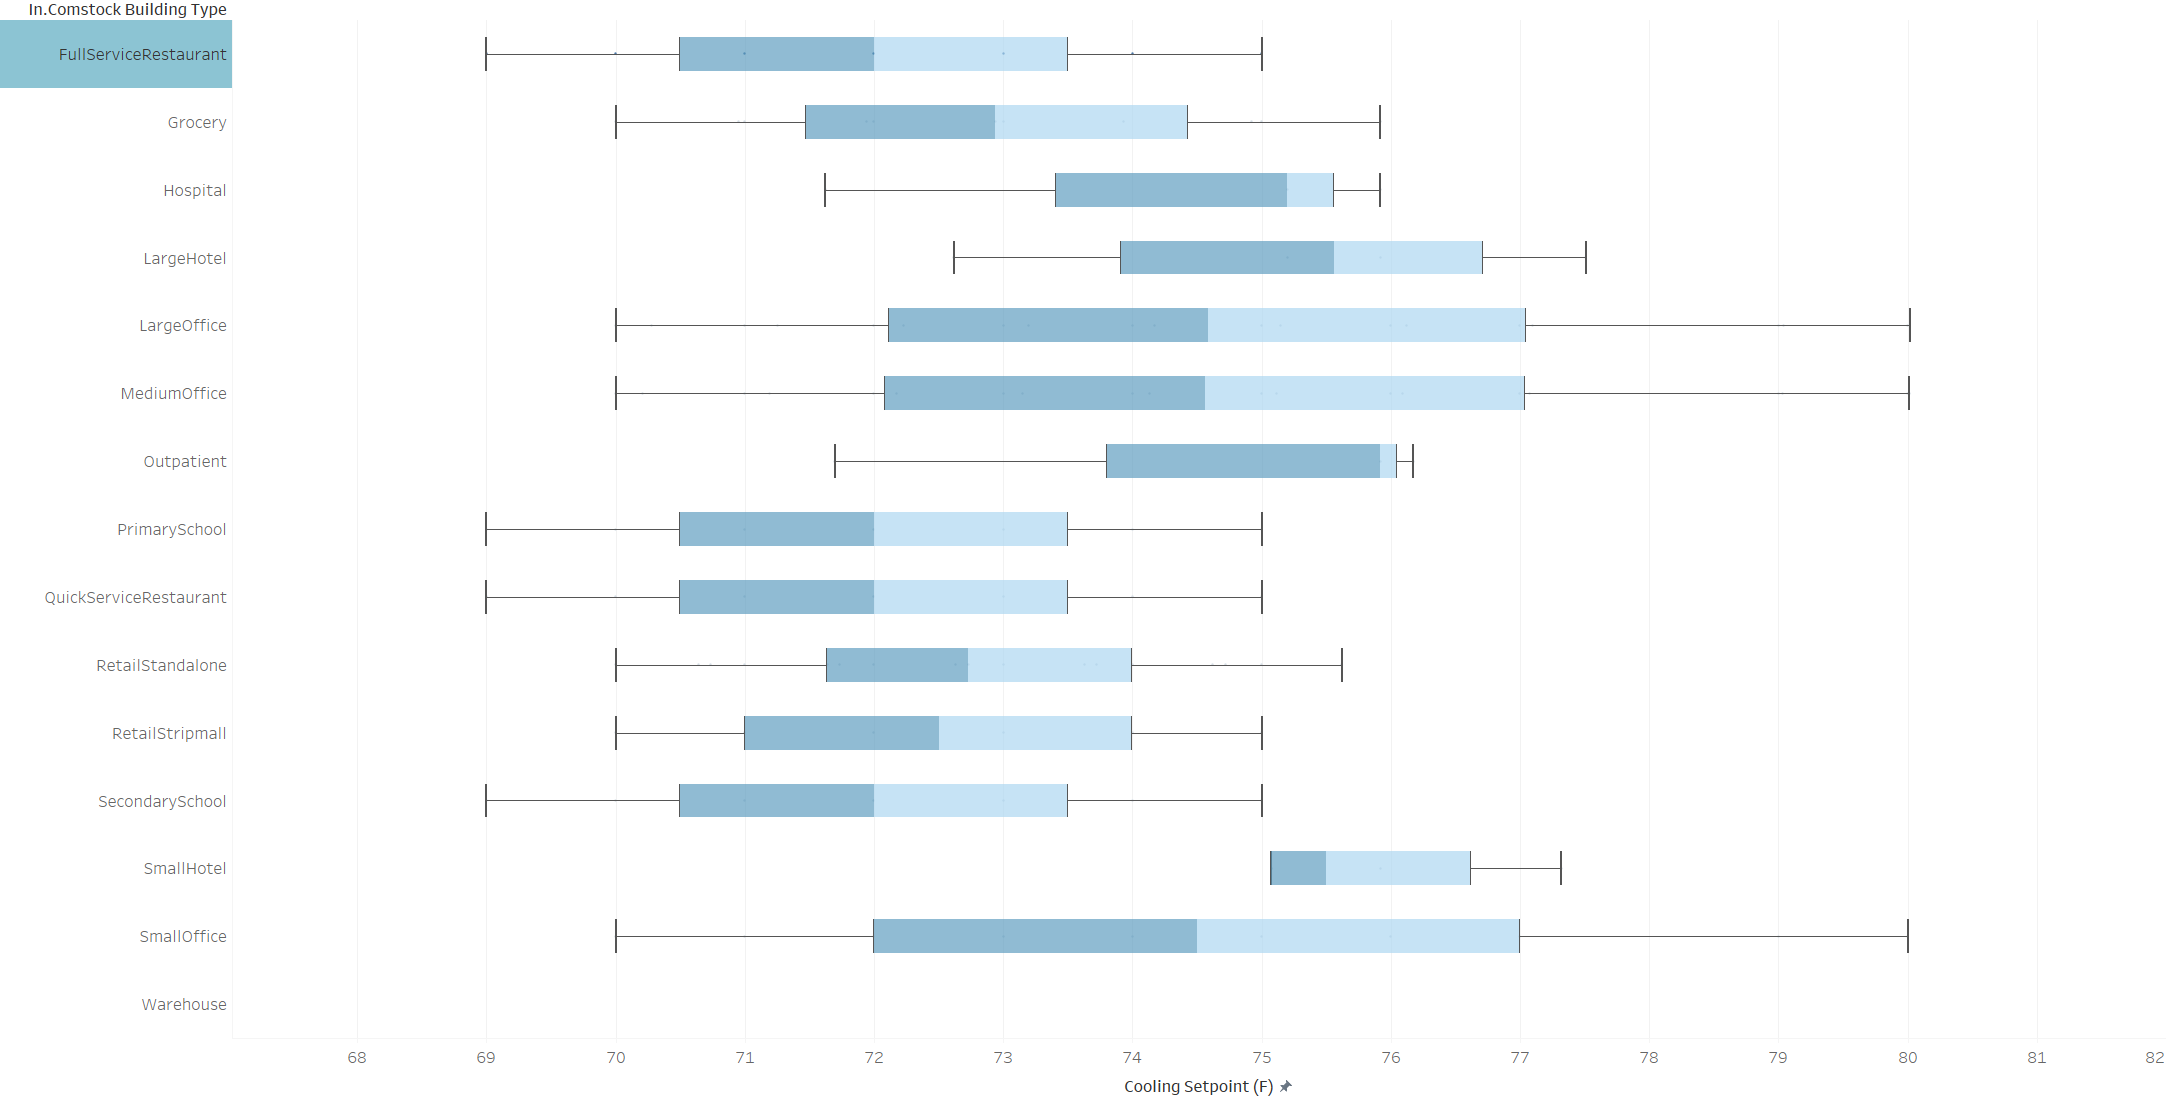
\includegraphics[width=1.0\textwidth]{figures/cooling_setpoints.png}
    \caption{Cooling thermostat set point (Fahrenheit) distributions per building type.}
    \label{fig:clg_therm_setpoints}
\end{figure}

\pagebreak
\subsubsection{Unoccupied Thermostat Setbacks}

An unoccupied thermostat setback defines the difference in the temperature set point from the occupied thermostat set point, for either heating or cooling, which is used during periods where the building is unoccupied. For example, an office might have an occupied heating set point of 71°F, but an unoccupied thermostat setback of 6°F for when the building is unoccupied, resulting in an unoccupied thermostat set point of 65°F (71°F - 6°F). This setback would be expected to save HVAC energy by relaxing the temperature requirements when there are no occupants in the building. This section describes ComStock's methodology for assigning unoccupied thermostat setback prevalence, as well as the setback temperature delta, for both heating and cooling.

The prevalence of thermostat setbacks in ComStock models is determined by building type using CBECS 2012. Each building type has some fraction of buildings with a thermostat setback, and some fraction without. The CBECS survey does not provide details on thermostat set point and setback temperatures, but it does provide survey responses as to whether heating and cooling setbacks are used, and whether these setbacks are manual. The survey responses are summarized by building type in Figure~\ref{fig:cbecs_therm_setback_summary}. However, it seems likely that many respondents who claim to implement manual setbacks do not reliably do so; we made a conservative assumption that only 20\% of manual setbacks would be counted as reliably practicing thermostat setbacks (manually adjusting the thermostat every night before leaving and every morning upon entering). The fraction of ComStock models that include thermostat setbacks is shown in Table~\ref{tab:thermostat_setback_prev}. Note that the timing of the thermostat setbacks coincides with the assigned hours of operation for a specific model, the methodology for which is described in Section~\ref{sec:hoo}.

\medskip
\begin{table}
\centering
\small
\caption[Fraction of ComStock Buildings with Thermostat Setbacks]{Fraction of ComStock Buildings With Thermostat Setbacks by Building Type}
\label{tab:thermostat_setback_prev}
\begin{tabular}{|l|l|}
\hline
\textbf{Building Type}          & \textbf{Fraction of Models With Thermostat Setback} \\ \hline
FullServiceRestaurant  & 0.57                                                \\ \hline
LargeOffice            & 0.77                                                \\ \hline
MediumOffice           & 0.76                                                \\ \hline
PrimarySchool          & 0.9                                                 \\ \hline
QuickServiceRestaurant & 0.46                                                \\ \hline
RetailStandalone       & 0.63                                                \\ \hline
RetailStripmall        & 0.9                                                 \\ \hline
SecondarySchool        & 0.95                                                \\ \hline
SmallOffice            & 0.77                                                \\ \hline
Warehouse              & 0.56                                                \\ \hline
\end{tabular}
\end{table}

\subsubsection{Unoccupied Thermostat Setbacks Informed by Building Automation System Data}

The method for determining the magnitude of the temperature setback for buildings with unoccupied temperature setbacks is described in this section. This methodology is used for the following building types: full service restaurant, large office, medium office, primary school, quick service restaurant, retail standalone, retail strip mall, secondary school, small office, and warehouse.

The magnitudes of the temperature setbacks are determined using the same data sets and methods described in Section~\ref{section:therm_setpoints_bas} for thermostat set points; probability distributions are created for each building type. The relationship between the thermostat set points and the delta setbacks is shown in Figure~\ref{fig:therm_setpoint_setback}. The resulting heating and cooling thermostat delta setback temperature probability distributions, for each applicable building type, are shown in Figure~\ref{fig:therm_heating_setback} and Figure~\ref{fig:therm_cooling_setback}, respectively.

\begin{figure}
    \centering 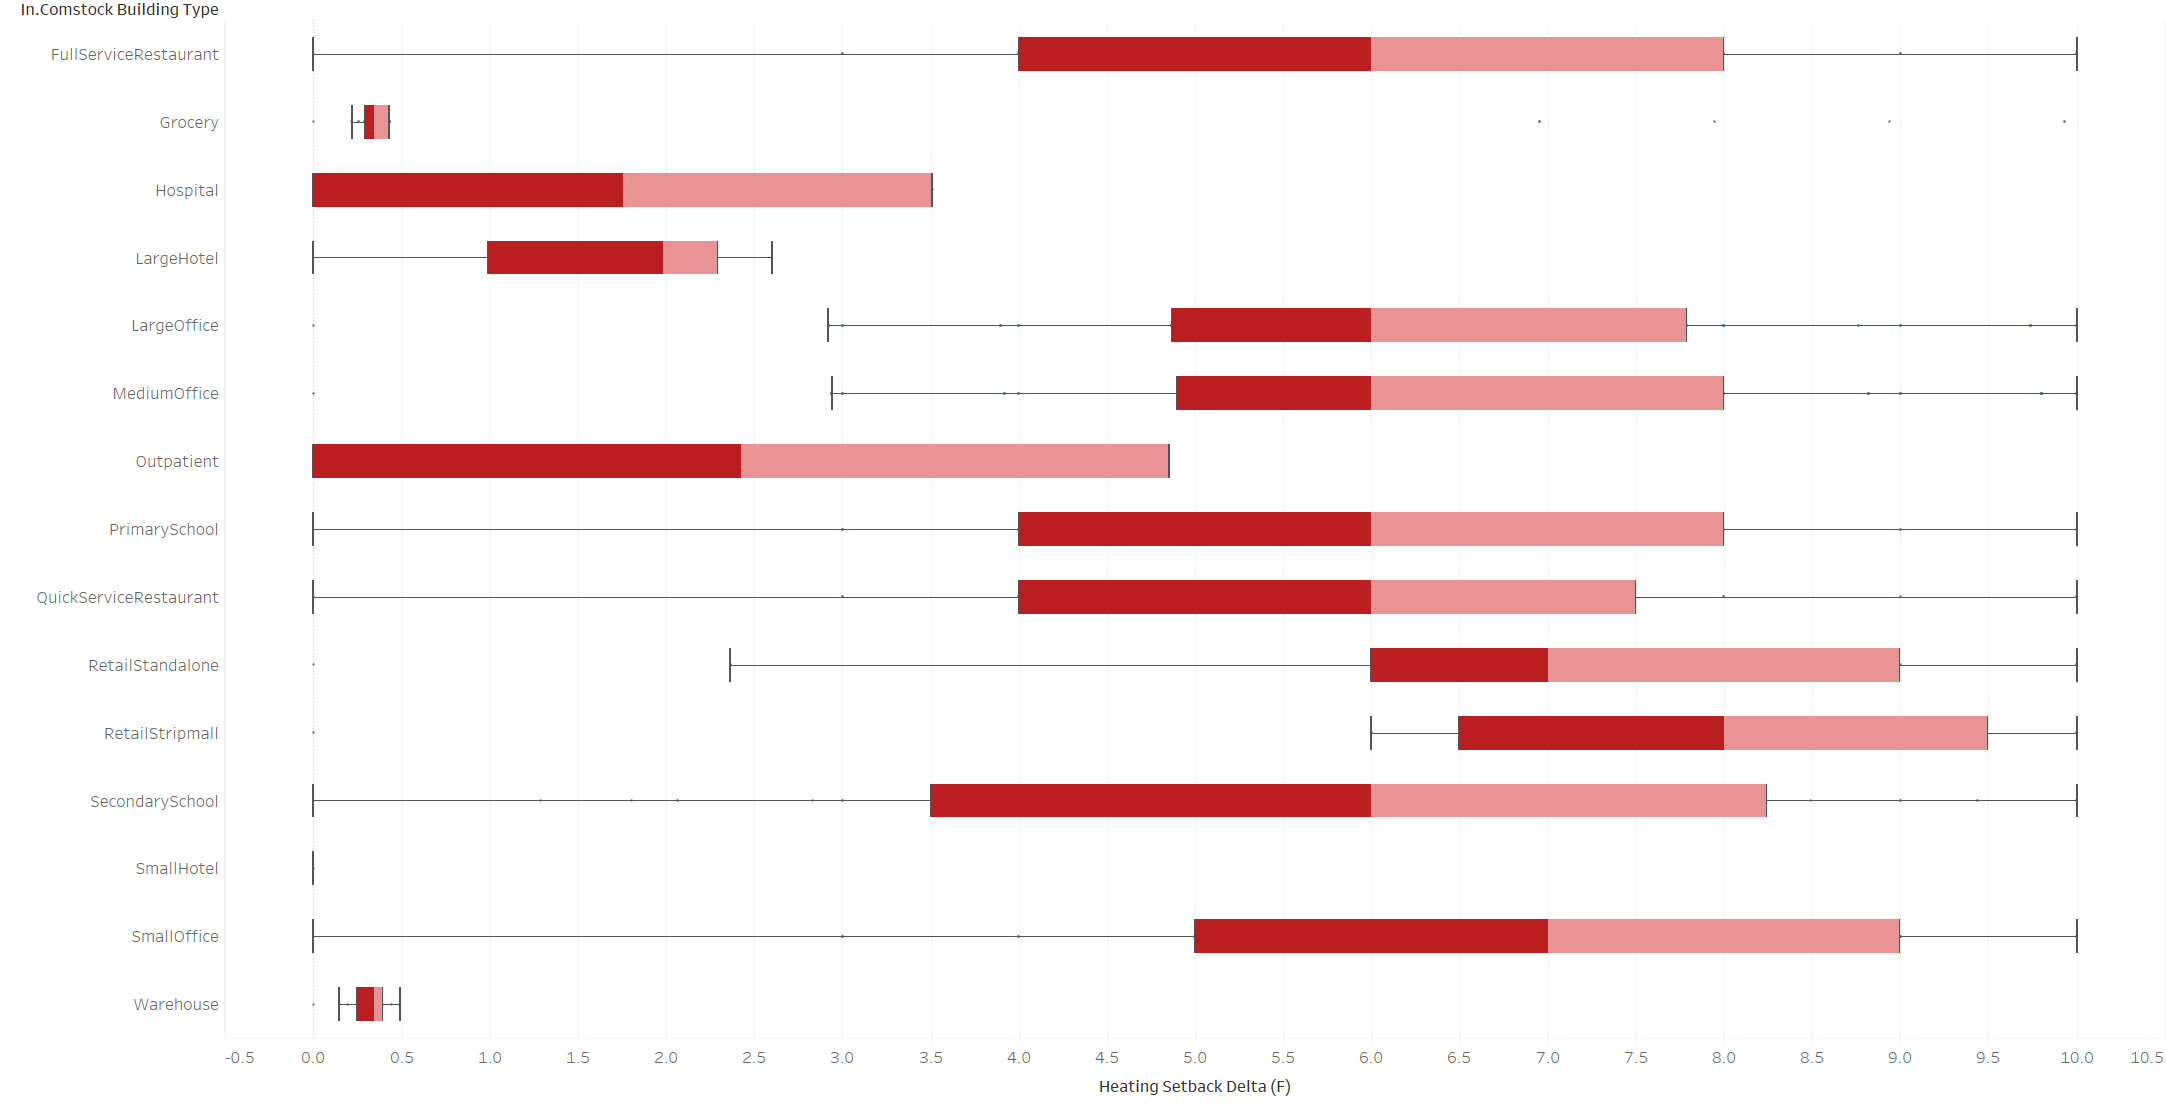
\includegraphics[width=1.0\textwidth]{figures/heating_setbacks.png}
    \caption{Thermostat heating setback delta temperature probability distributions per building type.}
    \label{fig:therm_heating_setback}
\end{figure}

\begin{figure}
    \centering 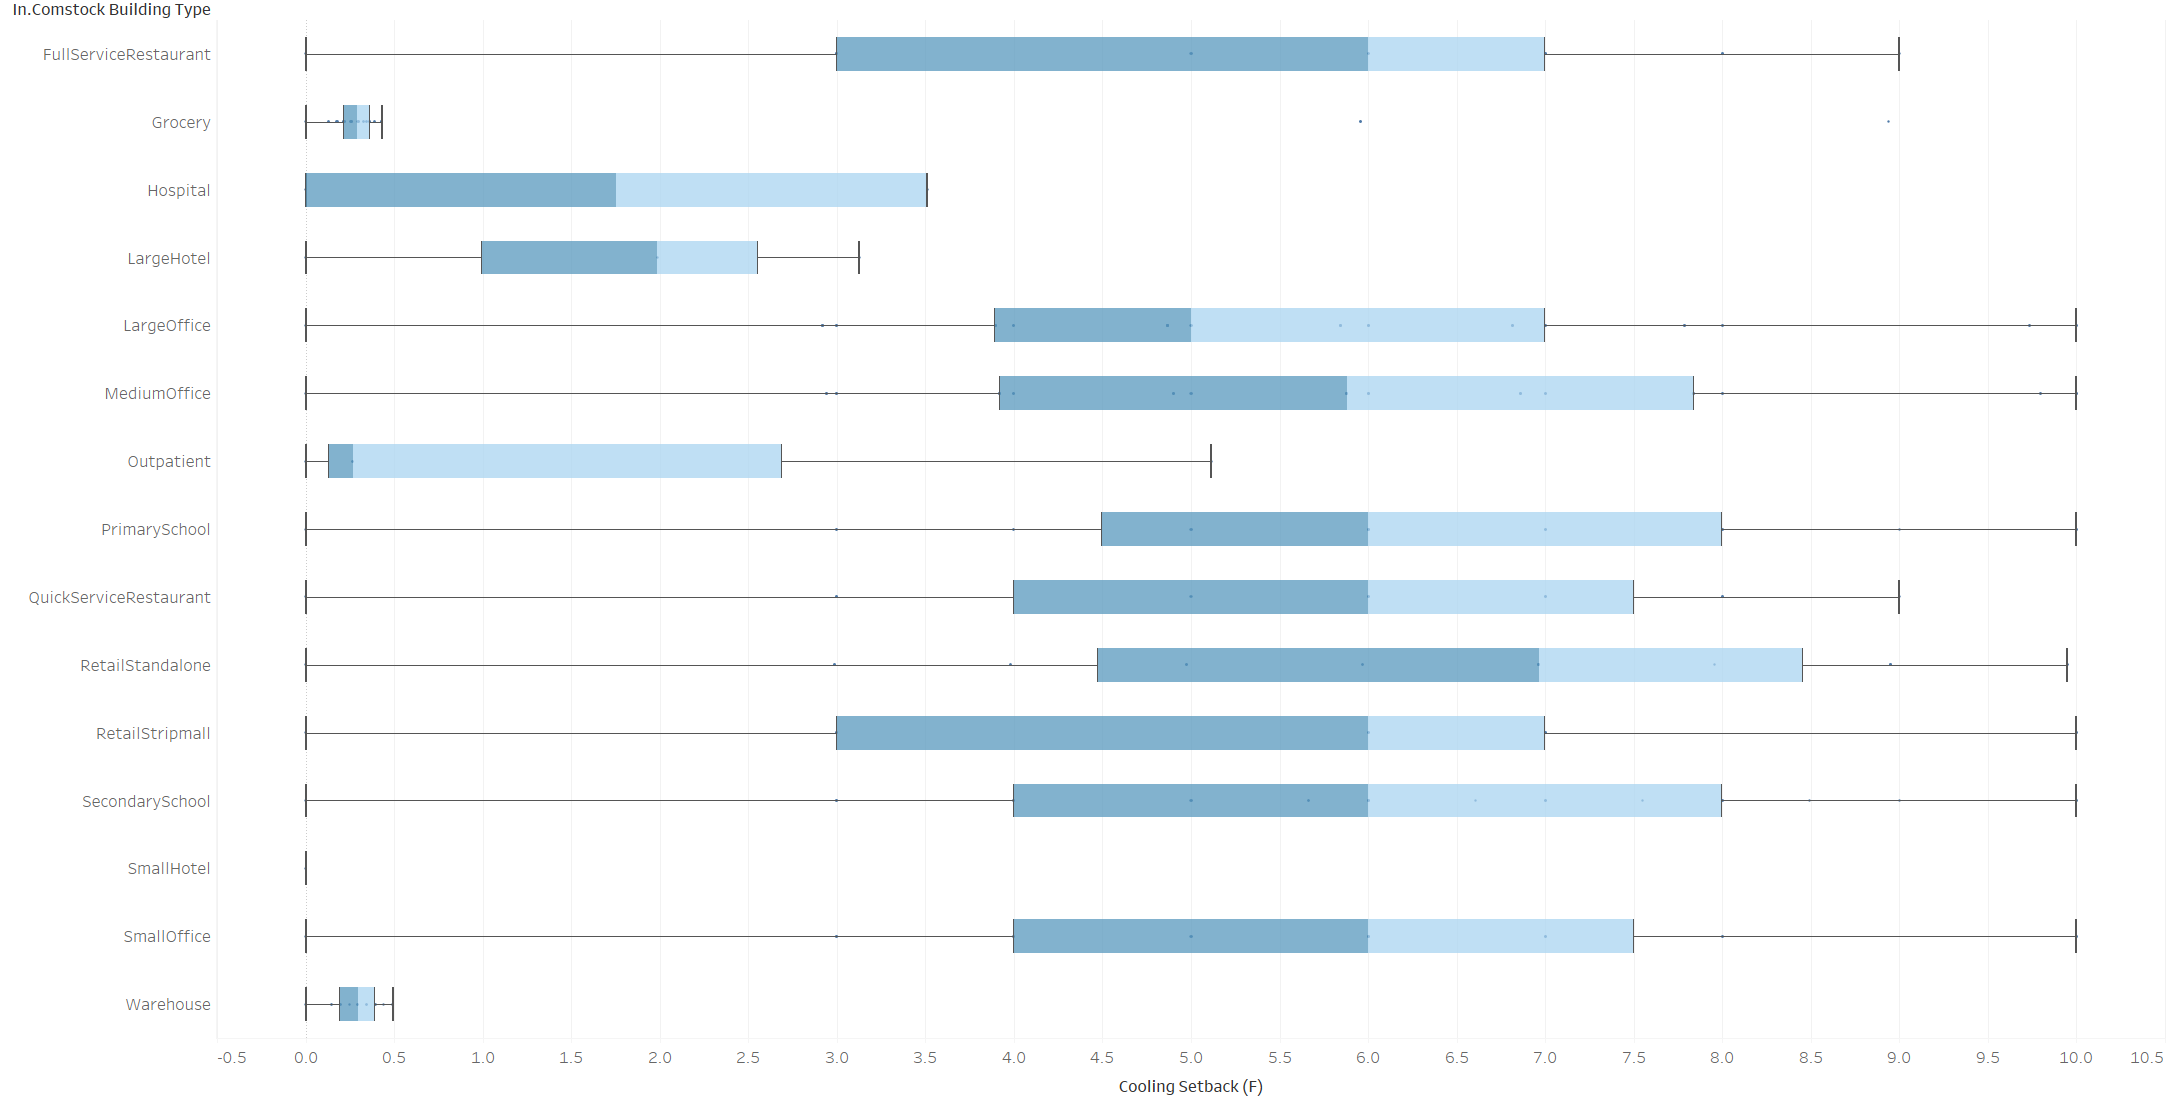
\includegraphics[width=1.0\textwidth]{figures/cooling_setbacks.png}
    \caption{Thermostat cooling setback delta temperature probability distributions per building type.}
    \label{fig:therm_cooling_setback}
\end{figure}

%\subsubsection{Thermostat Setpoints Not Informed by Building %Automation System Data}
% TODO: All of these alternative building types
%The following ComStock building types do not infer thermostat %setpoints from the BAS data, and therefore each have there own %methodology described in this section: Hospitals, Outpatient, %Warehouses, Small Hotels, and Large Hotels.
%\paragraph{Hospitals}
%\paragraph{Outpatient}
%\paragraph{Warehouses}
%\paragraph{Small Hotels}
%\paragraph{Large Hotels}

\pagebreak
\subsection{Unoccupied Air Handling Unit Operation}
\label{sec:unoccupied_ahu_operation}

Commercial buildings require constant design outdoor air ventilation rates when the building is occupied per ASHRAE-90.1. For air handling units (AHUs), the outdoor air is generally mixed with the supply air. This requires constant supply fan operation to maintain the outdoor air requirements established by ASHRAE-62.1 \citep{ashrae_62.1_2004}. However, AHUs do not need to provide outdoor ventilation air when the building is unoccupied. Therefore, ASHRAE-90.1 requires outdoor air dampers to close when the building is unoccupied, and to only cycle on supply fans as needed to maintain thermostat set points. This control scheme can have a large impact on energy usage, and data suggests that not all buildings implement these controls in their AHU systems. This section discusses ComStock's methodology for including the prevalence of different unoccupied AHU control schemes observed in real buildings, which follows the methodology used in \cite{unocc_hvac_paper}.

An industry-provided BAS data set of over 5,700 AHUs was used to inform the prevalence of three unoccupied AHU operation modes. The data set includes time series (hourly) BAS variables for ``Occupied Status'' (describes whether the AHU was in an occupied mode for that hour), ``Fan Status'' (describes whether the fan was used for that hour), and ``Ventilation Status'' (describes whether outdoor ventilation air was used for that hour). Counts of AHUs and buildings by building type in the data set are shown in Table~\ref{tab:unnoc_ahu_data_counts}, and the three unoccupied AHU shutdown control schemes are summarized in Table~\ref{tab:unnoc_ahu_schemes}.

The data set suggests that 27\% of AHUs use scheme 1 (least efficient), 50\% of AHUs use scheme 2 (more efficient), and 23\% of AHUs use scheme 3 (most efficient; ASHRAE-90.1 required). The prevalence of the AHU unoccupied control schemes by building type is shown in Table~\ref{tab:unnoc_ahu_scheme_prev}. These probability distributions are used in ComStock sampling to set the fraction of buildings utilizing the discussed control schemes, by building type, for models that use AHU-based HVAC systems. Non-AHU HVAC system types are not applicable to this methodology, nor are building types not listed in Table~\ref{tab:unnoc_ahu_scheme_prev}. Note that building types with less than 25 buildings in the BAS data set (Table~\ref{tab:unnoc_ahu_data_counts}) use the ``All Types'' distribution of the data set at large, as fewer than 25 samples cannot reliably be used to represent a population.

The following building types are not included in the unnocupied air handling unit operation workflow, and utilize default scheduling only: small hotels, large hotels, outpatient, hospitals, primary schools, and secondary schools. The building types may be integrated into this workflow in the future as more data becomes available.

\begin{table}[h!]
\centering
\small
\caption{Site and AHU Counts of Time Series BAS Data per Building Type}
\label{tab:unnoc_ahu_data_counts}
\begin{tabular}{|l|l|l|}
\hline
\textbf{Building Type} & \textbf{Site   Count} & \textbf{AHU   Count} \\ \hline
\textbf{All Types}     & 843                   & 5,706                \\ \hline
\textbf{Retail}        & 541                   & 3,300                \\ \hline
\textbf{Unknown}       & 164                   & 1,391                \\ \hline
\textbf{Office}        & 43                    & 466                  \\ \hline
\textbf{Restaurant}    & 39                    & 155                  \\ \hline
\textbf{Grocery}       & 35                    & 212                  \\ \hline
\textbf{Hotel}         & 6                     & 46                   \\ \hline
\textbf{Education}     & 6                     & 29                   \\ \hline
\textbf{Warehouse}     & 5                     & 94                   \\ \hline
\textbf{Healthcare}    & 4                     & 13                   \\ \hline
\end{tabular}
\end{table}
\begin{table}[h!]
\centering
\caption{AHU Operating Mode Schemes Used During Scheduled Unoccupied Times}
\label{tab:unnoc_ahu_schemes}
\begin{tabular}{|p{2.2cm}|p{4cm}|p{2cm}|p{2cm}|p{2cm}|p{2cm}|}
\hline
\textbf{Scheme Name} &
  \textbf{Unoccupied Control Scheme Description} &
  \textbf{Expected Efficiency} &
  \textbf{Occupied Status} &
  \textbf{Fan Status} &
  \textbf{Ventilation Status} \\ \hline
\textbf{Scheme 1} & Scheduled on, running                                                            & Least Efficient & Active   & Active & Active   \\ \hline
\textbf{Scheme 2} & Scheduled off, fan cycles with ventilation to maintain thermostat   setpoints    & More Efficient  & Inactive & Active & Active   \\ \hline
\textbf{Scheme 3} & Scheduled off, fan cycles without ventilation to maintain thermostat   setpoints & Most Efficient  & Inactive & Active & Inactive \\ \hline
\end{tabular}
\end{table}

\subsection{Demand Control Ventilation}

Demand control ventilation (DCV) acts to reduce outdoor air ventilation during periods of detected low occupancy. Occupancy levels are generally detected through the use of CO\textsubscript{2} sensors located directly in the space or within the HVAC system.

DCV is included in ComStock models when required by the governing ASHRAE-90.1 energy code for the specific spaces/systems in the model. ComStock gathers the necessary criteria for determining DCV requirements and includes DCV functionality only if the space/system requires it. The requirement criteria for DCV include space floor area, space design occupant density, system economizer prevalence, system design outdoor air flow rate, and system energy recovery prevalence. The 90.1 code year for a model is based on the year of the model's last major HVAC replacement. Code year assignment and system turnover assumptions are described further in Section \ref{sec:system_turnover_and_eul}. A summary of the floor area served by a system with DCV is shown in Table~\ref{tab:dcv_prev}. Note that DCV is not required by ASHRAE 90.1 when an HVAC system has an ERV. One important observation from these data is that no office buildings include DCV. This is because office buildings are currently modeled using a single, blended space type that is a fractional mix of open offices, enclosed offices, conference rooms, etc. The occupancy density of this blended space does not exceed the DCV thresholds in ASHRAE 90.1. This leads to unrealistically low (0\%) DCV in office buildings. Another important observation is that DCV is not modeled in any of the buildings in California (which use the DEER data set), although this does not align with the newer versions of Title 24. DCV is expected to be implemented in California buildings in the near future.
%NOTE: DCV table does not look good. Nothing for DEER. Inconsistent for code years. Nothing for offices.
%TODO: DIscuss DCV excemptions, such as ERV prev


\subsection{Air-Side Energy Recovery}
\label{sec:erv}

Energy recovery ventilators (ERVs) in AHUs reduce energy consumption by pre-conditioning the incoming outdoor air using the system exhaust air, which reduces the heating and cooling energy required to condition the air. Energy recovery is especially effective in systems serving spaces with high outdoor air ventilation loads.

ERVs are included in ComStock model HVAC systems only when required by the governing energy code for the specific system. This determination is made using OpenStudio-Standards, where the necessary ComStock model properties are gathered to determine whether an ERV is required for each system. These properties include the climate zone, percent outdoor air, and design supply airflow rate, aligning with ASHRAE-90.1 Table 6.5.6.1 for the respective energy code year followed. A summary of the floor area served by systems with energy recovery is shown in Table~\ref{tab:energy_recovery_prev}.

%TODO: Discuss ERV wheel power methodology

\begin{table}[h!]
\centering
\scriptsize
\caption[Energy Recovery Prevalence]{Fraction of Floor Area Served by HVAC Systems With Energy Recovery by Building Type and Code Year}
\label{tab:energy_recovery_prev}
\begin{tabular}{|p{2.2cm}|p{0.3in}|p{0.3in}|p{0.3in}|p{0.3in}|p{0.3in}|p{0.3in}|p{0.3in}|}
\hline
\textbf{Building Type} &
  \textbf{Pre-1980} &
  \textbf{1980--2004} &
  \textbf{90.1-2004} &
  \textbf{90.1-2007} &
  \textbf{90.1-2010} &
  \textbf{90.1-2013} &
  \textbf{DEER All Years} \\ \hline
FullService\-Restaurant  & 0 & 0 & 0.051 & 0.027 & 0.347 & 0.392 & 0 \\ \hline
Hospital               & 0 & 0 & 0.457 & 0.442 & 0.613 & 0.871 & 0 \\ \hline
LargeHotel             & 0 & 0 & 0.109 & 0.09  & 0.267 & 0.245 & 0 \\ \hline
LargeOffice            & 0 & 0 & 0.028 & 0.035 & 0.139 & 0.519 & 0 \\ \hline
MediumOffice           & 0 & 0 & 0.007 & 0.016 & 0.093 & 0.306 & 0 \\ \hline
Outpatient             & 0 & 0 & 0.087 & 0.078 & 0.095 & 0.246 & 0 \\ \hline
PrimarySchool          & 0 & 0 & 0.376 & 0.41  & 0.597 & 0.639 & 0 \\ \hline
QuickService\-Restaurant & 0 & 0 & 0     & 0     & 0.088 & 0.063 & 0 \\ \hline
RetailStandalone       & 0 & 0 & 0.027 & 0.022 & 0.029 & 0.306 & 0 \\ \hline
RetailStripmall        & 0 & 0 & 0.115 & 0.111 & 0.191 & 0.435 & 0 \\ \hline
SecondarySchool        & 0 & 0 & 0.540 & 0.530 & 0.675 & 0.725 & 0 \\ \hline
SmallHotel             & 0 & 0 & 0.186 & 0     & 0.092 & 0     & 0 \\ \hline
SmallOffice            & 0 & 0 & 0     & 0     & 0.044 & 0.050 & 0 \\ \hline
Warehouse              & 0 & 0 & 0.065 & 0.053 & 0.069 & 0.083 & 0 \\ \hline
\end{tabular}
\end{table}

An enthalpy wheel ERV system (rotary) is added to the HVAC systems in ComStock models where an ERV is determined to be required. The effectiveness of the system is 50\% for all conditions, aligning with the requirements of ASHRAE-90.1. Economizer lockout and supply air bypass for temperature control are included. The defrost type is exhaust only, which temporarily bypasses the supply side of the heat exchanger to allow warmer exhaust air to remove frost uninhibited when needed.

\subsection{Air-Side Economizers}

Air-side economizers reduce HVAC cooling energy by increasing the amount of outdoor ventilation air during times when the temperature and/or enthalpy are beneficial for cooling. For example, if the outdoor air temperature is 55°F when the building needs cooling, the HVAC system can increase the amount of outdoor ventilation air being delivered to the space to satisfy some or all of the cooling requirement in place of mechanical cooling.

As described in Section~\ref{sec:system_turnover_and_eul}, we assume that some building systems, including the HVAC system, are replaced over the lifespan of the building. We re-evaluate the requirement for an air-side economizer based on the energy code in force at the time of the latest HVAC system replacement. For buildings outside of CA, energy code requirements were taken from ASHRAE 90.1. For buildings inside CA, the CA energy code requirements were evaluated taken from the CA DEER MASControl3 models \citep{mascontrol3}, where the economizer limits and applicability were found as shown in Table~\ref{tab:econ_lims_mascontrol3} and Table~\ref{tab:econ_applic_mascontrol3}.

\begin{table}[h!]
  \centering
  \small
  \caption[MASControl3 Economizer Limits]{Economizer limits from MASControl3}
  \label{tab:econ_lims_mascontrol3}
  \begin{tabular}{|p{0.75in}|p{1.25in}|p{1.5in}|}
  \hline
  \textbf{Climate Zone} &
  \textbf{Drybulb Limit (°F)} &
  \textbf{Enthalpy Limit (Btu/lb)} \\ \hline
  CZ01 & 70 & 28 \\ \hline
  CZ02 & 73 & 28 \\ \hline
  CZ03 & 70 & 28 \\ \hline
  CZ04 & 73 & 28 \\ \hline
  CZ05 & 70 & 28 \\ \hline
  CZ06 & 71 & 28 \\ \hline
  CZ07 & 69 & 28 \\ \hline
  CZ08 & 71 & 28 \\ \hline
  CZ09 & 71 & 28 \\ \hline
  CZ10 & 73 & 28 \\ \hline
  CZ11 & 75 & 28 \\ \hline
  CZ12 & 75 & 28 \\ \hline
  CZ13 & 75 & 28 \\ \hline
  CZ14 & 75 & 28 \\ \hline
  CZ15 & 75 & 28 \\ \hline
  CZ16 & 75 & 28 \\ \hline
  \end{tabular}
  \end{table}

\begin{table}[h!]
  \centering
  \small
  \caption[MASControl3 Economizer Applicability]{Economizer applicability from MASControl3}
  \label{tab:econ_applic_mascontrol3}
  \begin{tabular}{|p{0.75in}|p{1in}|p{1in}|p{1in}|}
  \hline
  \textbf{Vintage} &
  \textbf{Packaged DX} &
  \textbf{Chilled Water} &
  \textbf{Water Loop HP} \\ \hline
  1975  & FALSE & TRUE & FALSE \\ \hline
  1985  & FALSE & TRUE & FALSE \\ \hline
  ~1996 & FALSE & TRUE & FALSE \\ \hline
  2003  & FALSE & TRUE & FALSE \\ \hline
  2007  & FALSE & TRUE & FALSE \\ \hline
  2011  & FALSE & TRUE & FALSE \\ \hline
  2014  & TRUE  & TRUE & TRUE  \\ \hline
  2015  & TRUE  & TRUE & TRUE  \\ \hline
  2017  & TRUE  & TRUE & TRUE  \\ \hline
  2020  & TRUE  & TRUE & TRUE  \\ \hline
  \end{tabular}
  \end{table}

Figure~\ref{fig:economizer_presence} shows the prevalence of economizers (in terms of floor area coverage and contribution to cooling energy) for different subcategories (building type and ventilation system type) of the existing building stock. The percentage of floor area where "economizer availability" is "True" includes the total building area if there is at least one economizer in the building. It does not represent the total floor area served by systems with economizers. While there are buildings that already include economizers in variable air volume (VAV) systems and roof top units (RTU) covering 40\% of the total floor area and 28\% of total electricity used for cooling, the remaining portion of buildings with those system types do not include economizers.

\begin{figure}
  \centering 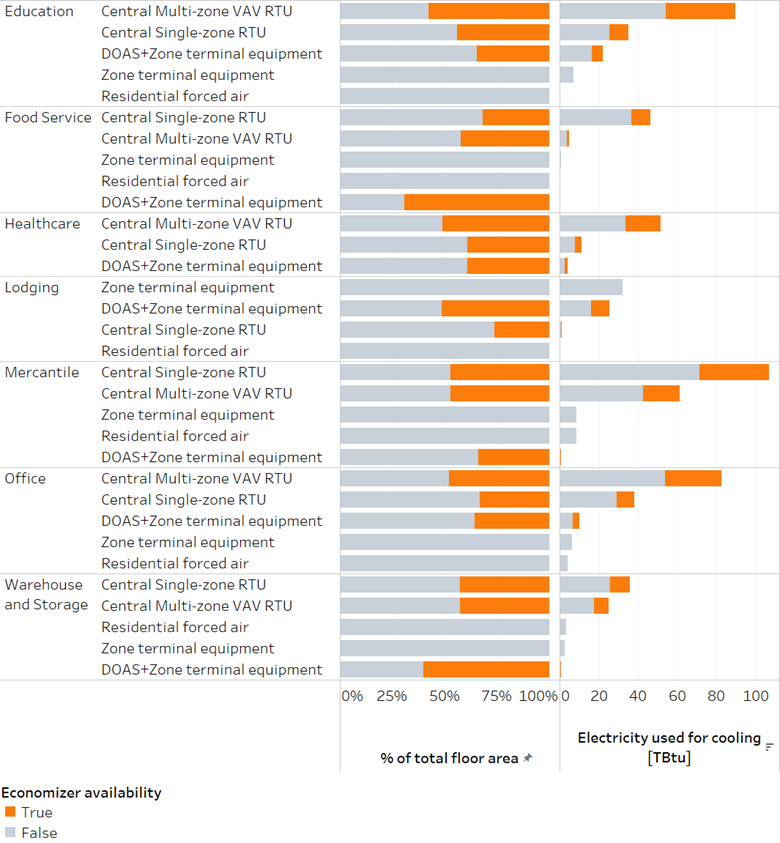
\includegraphics[width=0.7\textwidth]{figures/economizer_presence.png}
  \caption{Presence of air-side economizers in the building stock.}
  \label{fig:economizer_presence}
\end{figure}

Based on a large body of anecdotal evidence from conversations with fault-focused field engineers and a brief review of common current (Trane, Carrier, Daikin) rooftop unit product data sheets \citep{trane_foundation}, \citep{carrier_economiser}, \citep{daikin_rebel}, fixed dry bulb controls are a more common choice than differential dry bulb controls, although manufacturers also offer dual enthalpy (fixed dry bulb + fixed enthalpy) options with the addition of an enthalpy sensor. For this reason, fixed dry bulb controls are assumed for almost all building vintages and climate zones, with the exception being ASHRAE 90.1-2010 and 2013, which prohibited fixed dry bulb economizers in the warmer humid climate zones. These restrictions were lifted in ASHRAE 90.1-2016.

Figure~\ref{fig:economizer_prevalence} shows the comparison of economizer coverage with respect to building floor area between ComStock and estimation from Commercial Buildings Energy Consumption Survey \citep{eia2018cbecs}. Because of how data is structured in CBECS, the floor area shown in these figures represents the entire floor area of the building if any economizer is present in any of the HVAC systems in the building rather than actual floor area covered by HVAC systems with an economizer. Because CBECS data only shows total building area instead of total area covered by the economizers, this comparison helps give a rough estimate of economizers.

\begin{figure}
  \centering 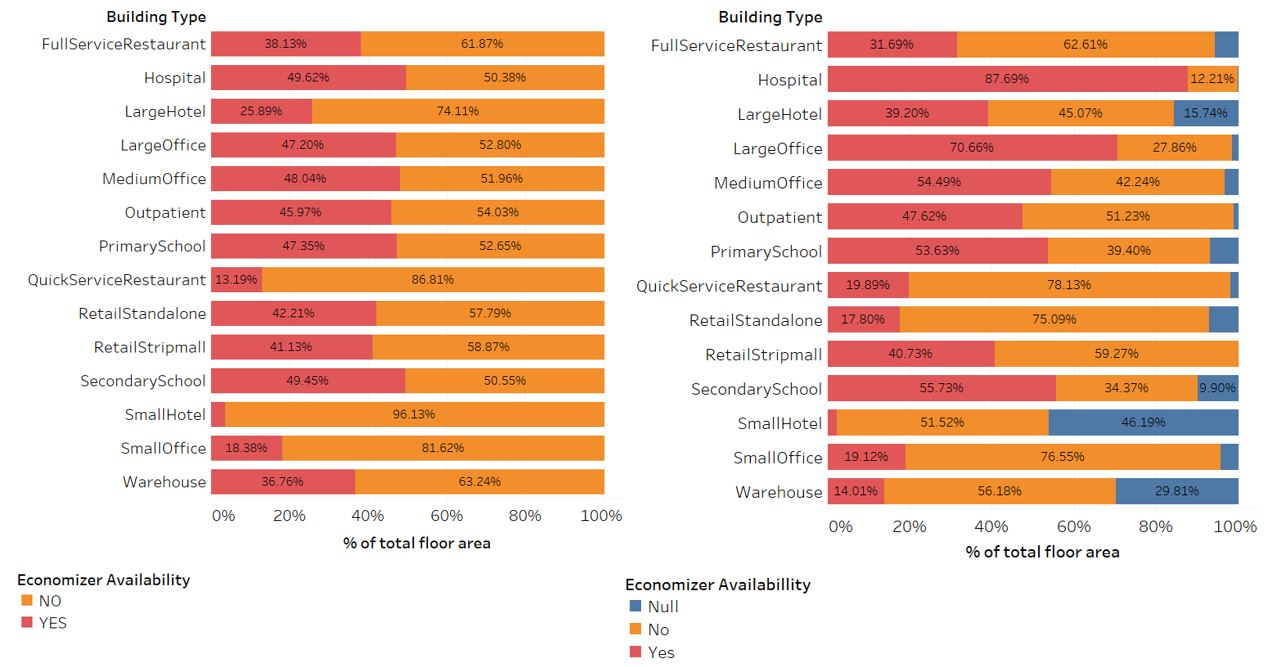
\includegraphics[width=0.7\textwidth]{figures/economizer_prevalence.png}
  \caption{Economizer floor area coverage comparing ComStock (left) with CBECS 2018 (right).}
  \label{fig:economizer_prevalence}
\end{figure}

Economizers are well known for frequent faulty operations. There were many efforts in the past to understand fault characteristics in commercial buildings \citep{doi_10_1080_23744731_2021_1898243}, \citep{osti_1889192}, \citep{osti_1829706}, \citep{osti_1457127}. While this evidence is insufficient to reflect all aspects (e.g., prevalence, incidence, intensity, and evolution described in \citep{doi_10_1080_23744731_2021_1898243}) of all faults in the commercial building stock across the country, it is possible to make simplifications for modeling certain fault types based on available data.

Figure~\ref{fig:econ_temp_fault} shows how the first fault is modeled for buildings with economizers. Crowe et al. \citep{osti_1889192} acquired data from AFDD venders that monitored 3,660 AHUs and 7,974 RTUs and reported 31\% of all economizers were experiencing faulty operations. Shoukas et al. \citep{osti_1665808} received data from a clothing retailer and food chain that monitored 1,416 RTUs and reported 60\% of all faults related to economizers were related to economizer not effectively reducing cooling load compared to the theoretical potential. The symptom described as "ineffective economizing" can be due to different faults: damper stuck, damper bias, sensor bias, sensor frozen, inappropriate configuration, etc. A report \citep{seventhwave_rtu} published by Minnesota Department of Commerce Division of Energy Resources monitored 41 RTUs in Minnesota that were installed in many different building types (e.g., office, restaurant, retail, hotel, etc.) and reported the actual changeover temperature setting in the economizer were not configured efficiently (average of 52°F) resulting in missed free cooling opportunity.

Based on this information focusing on different aspects of the fault, a fault measure was developed as shown in Figure~\ref{fig:econ_temp_fault}. The figure includes a description of the fault as well as four different metrics that define the characteristics of a fault. Fault intensity (or severity) is when a fault can have a severity level. For example, if the sensor is drifting, the intensity is the difference between the true value and the biased measured value. Fault prevalence refers to the portion of systems or components with the fault among all systems or components in the sample space (e.g., 30\% of all economizers have the fault). Fault incidence refers to the occurrence rate of a fault for a given system or component over for a given time period (e.g., economizer damper gets stuck once every year). Fault evolution refers to certain faults where the severity naturally changes over time. For example, sensor drift is typically a fault where the severity changes over the course of time. For the incorrect high limit setting described in Figure~\ref{fig:econ_temp_fault}, the fault changes the changeover temperature setting of an economizer to 52°F and applies to 30\% of economizers that use fixed dry-bulb control. Fault incidence and fault evolution were not modeled because these aspects are mostly irrelevant for this fault.

\begin{figure}
  \centering 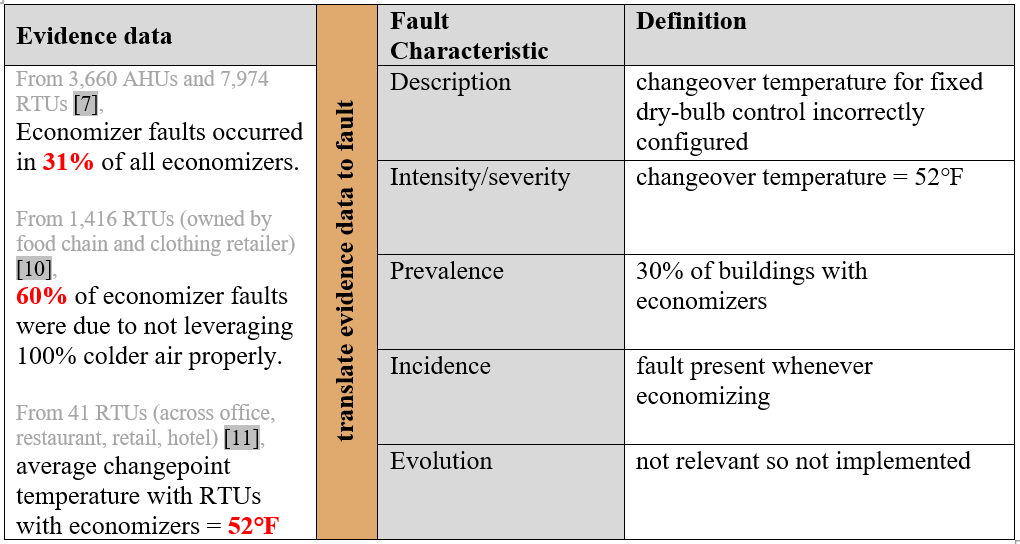
\includegraphics[width=0.7\textwidth]{figures/econ_temp_fault.png}
  \caption{Economizer incorrect changeover temperature setting fault description.}
  \label{fig:econ_temp_fault}
\end{figure}

Figure~\ref{fig:econ_temp_fault_single_model} shows a comparison of simulated operation with and without the fault. As a result, the fault will reduce the changeover (high limit) temperature of the economizer, disabling the economizer even if the outdoor air temperature is favorable (e.g., 52-72°F), thus, losing opportunities for free cooling. The figure shows how the fault impacts the annual cooling energy, how the changepoint temperature changes with fault, and how the transient response changes.

\begin{figure}
  \centering 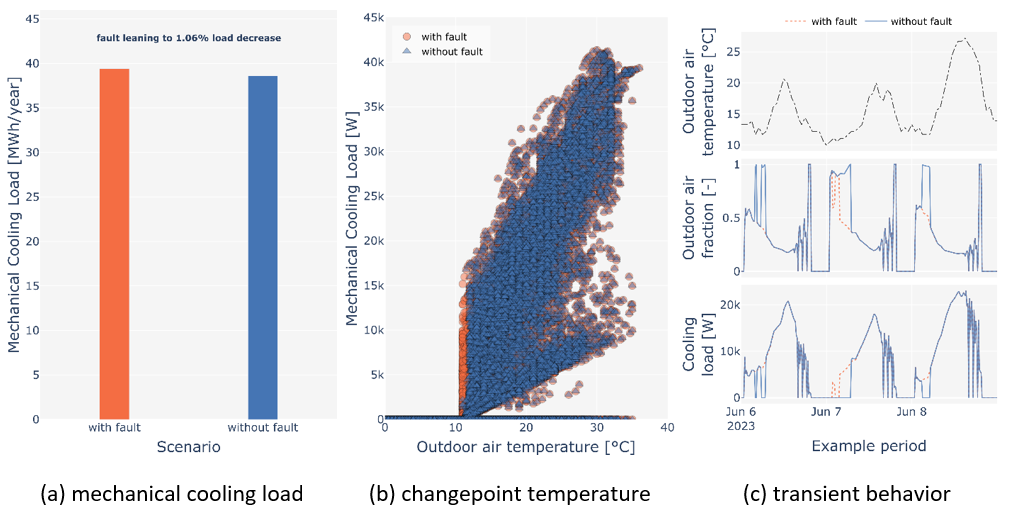
\includegraphics[width=0.7\textwidth]{figures/econ_temp_fault_single_model.png}
  \caption{Economizer incorrect changeover temperature setting fault impact on simulation results.}
  \label{fig:econ_temp_fault_single_model}
\end{figure}

As reported by Heinemeier \citep{heinemeier2014free}, contractors in California stated that 30-40\% of economizers they have worked with were disabled with fully closed dampers. This is often caused by mechanical linkage issues between damper and actuator, where the economizer automatically reverts to the fully closed position as a safety measure. An economizer with a fully closed damper will not draw any fresh outdoor air, causing an air quality issue. Depending on the outdoor air condition (i.e., favorable or not favorable for economizing), it can either reduce or increase energy consumption. Figure~\ref{fig:econ_damper_fault} shows the description of the fault for the economizer outdoor air damper fully closed and stuck. Unlike the fault described in Figure~\ref{fig:econ_temp_fault}, this fault has a bigger impact on air quality and energy and the incidence of the fault is important.

\begin{figure}
  \centering 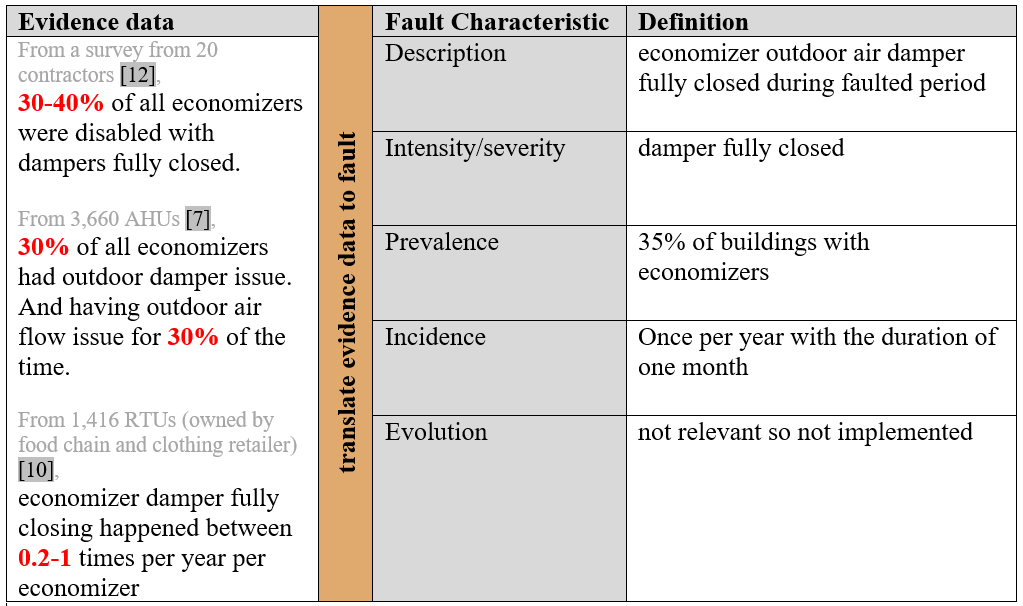
\includegraphics[width=0.7\textwidth]{figures/econ_damper_fault.png}
  \caption{Economizer damper stuck closed fault description.}
  \label{fig:econ_damper_fault}
\end{figure}

Figure~\ref{fig:econ_damper_fault_single_model} shows example simulation results for a building with and without the damper fully closed fault. The fault was imposed once during the entire April period resulting in 1.8\% mechanical load increase. As mentioned previously, the energy impact of the fault can either be increased or decreased energy consumption, and Figure~\ref{fig:econ_damper_fault_single_model}(c) highlights the transition from negative to positive savings when the outdoor air temperature transitions from favorable to unfavorable conditions.

\begin{figure}
  \centering 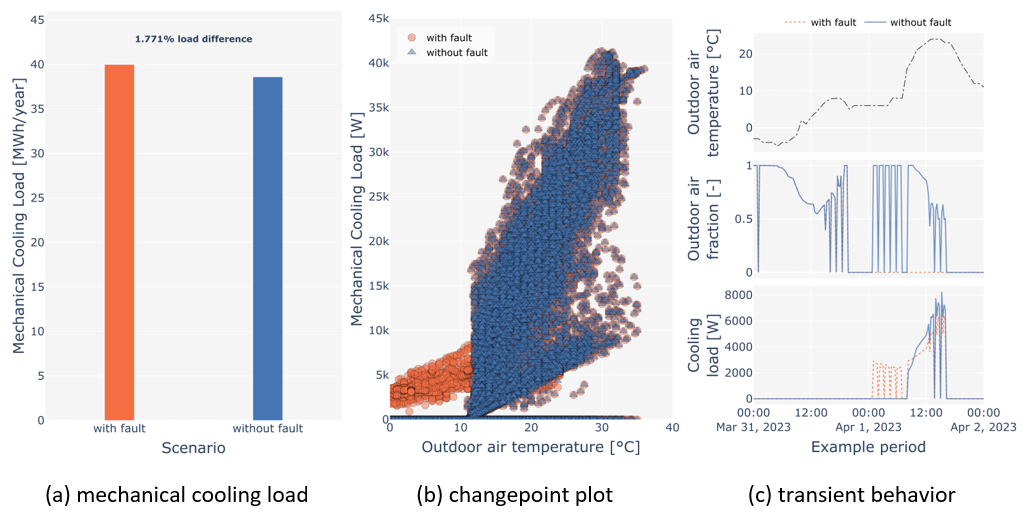
\includegraphics[width=0.7\textwidth]{figures/econ_damper_fault_single_model.png}
  \caption{Economizer damper stuck closed fault impact on simulation results.}
  \label{fig:econ_damper_fault_single_model}
\end{figure}

Although faults (e.g., damper fully closed) are implemented with fixed prevalence (e.g., 35\%), the actual percentage of economizers being faulted (among applicable economizers) is less than the defined prevalence due to implementation limitations. For example, 35\% of randomly selected buildings that include certain HVAC system types (categorized by the air system) are assigned the damper fully closed fault. However, certain portions of these air systems do not have economizers, thus, they cannot have an economizer fault. In other words, the current limitation is that the random selection of faulted economizers is not fully aligned with buildings that actually have economizers. In these cases, we are losing the opportunity for applying faults and decreasing the representation of fault prevalence in final building stock. Newer versions of California's Title 24 energy code requires fault detection and diagnostics (FDD) for economizers which should prevent and mitigate faults. However, ComStock does not reflect the impact of FDD technology, possibly overestimating the impact of faults in buildings with newer HVAC systems in California.

\subsection{Furnaces}

Furnaces are used in a variety of HVAC equipment for space heating through the direct combustion of a fuel. For ComStock models, the fuel type can be natural gas, propane, or fuel oil. The following ComStock system types use furnaces: direct evaporative coolers with forced air furnace, gas unit heaters, PSZ-AC with gas coil, PTAC with gas coil, residential AC with residential forced air furnace, and residential forced air furnace.

\subsubsection{Furnace Efficiencies}

Furnaces in ComStock are all assumed to be standard, non-condensing types at this time. Rated efficiency assignments are a function of capacity and in-force HVAC template code. The furnace efficiency assignments are summarized in Table~\ref{tab:furnace_eff_assignments}.

\subsubsection{Furnace Performance Modifiers}

Furnaces in ComStock do not use any performance curves, so there is no change in efficiency or capacity as a function of temperature or part load ratio, and therefore no cycling losses. Furthermore, no parasitic fuel losses are included in ComStock furnace models.

\begin{table}
\centering
\scriptsize
\caption[Furnace Efficiency]{Furnace Efficiency by Capacity and Code Year}
\label{tab:furnace_eff_assignments}
\begin{tabular}{|p{0.5in}|p{0.5in}|p{0.5in}|p{0.5in}|p{0.5in}|p{0.5in}|p{1.5in}|}
\hline
\textbf{Template} &
  \textbf{Minimum   Capacity (Btu/hr)} &
  \textbf{Maximum   Capacity (Btu/hr)} &
  \textbf{Minimum   Annual Fuel Utilization Efficiency (AFUE)} &
  \textbf{Minimum   Thermal Efficiency (\%)} &
  \textbf{Minimum   Combustion Efficiency (\%)} &
  \textbf{Notes} \\ \hline
Pre-1980  & -           & 249,999       & -    & 0.8 & -   & -                                        \\ \hline
Pre-1980  & 250,000     & no max & -    & 0.8 & -   & -                                        \\ \hline
Pre-1980  & 250,000,000 & no max & -    & 0.8 & -   & -                                        \\ \hline
1980--2004 & -           & 299,999       & -    & 0.8 & -   & -                                        \\ \hline
1980--2004 & 300,000     & 249,999,999   & -    & 0.8 & -   & -                                        \\ \hline
90.1-2004           & -           & 224,999       & 0.78 & 0.8 & -   & \multirow{10}{*}{\parbox{2.5cm}{Table   6.8.1E page 49}} \\ \cline{1-6}
90.1-2004           & 225,000     & 249,999,999   & -    &     & 0.8 &                                          \\ \cline{1-6}
90.1-2007           & -           & 224,999       & 0.78 & 0.8 & -   &                                          \\ \cline{1-6}
90.1-2007           & 225,000     & 249,999,999   & -    &     & 0.8 &                                          \\ \cline{1-6}
90.1-2010           & -           & 224,999       & 0.78 & 0.8 & -   &                                          \\ \cline{1-6}
90.1-2010           & 225,000     & 249,999,999   & -    & 0.8 & -   &                                          \\ \cline{1-6}
90.1-2013           & -           & 224,999       & 0.78 & 0.8 & -   &                                          \\ \cline{1-6}
90.1-2013           & 225,000     & 249,999,999   & -    & 0.8 & -   &                                          \\ \cline{1-6}
90.1-2016           & -           & 224,999       & 0.78 & 0.8 & -   &                                          \\ \cline{1-6}
90.1-2016           & 225,000     & 249,999,999   & -    & 0.8 & -   &                                          \\ \hline
90.1-2019           &  -          & 224,999       & -    & 0.81 &
  - &
  \multirow{2}{*}{\parbox{1.5in}{Table   6.8.1-6 for \textgreater 225 kBtu/hr; Table F-4 for \textless 225 kBtu/hr}} \\ \cline{1-6}
90.1-2019           & 225,000     & 249,999,999   & -    & 0.8 & -   &                                          \\ \hline
\end{tabular}
\end{table}

\subsection{Boilers}

Boilers create hot water for heating in buildings. The following ComStock HVAC types use boilers for heating: baseboard gas boiler, DOAS with fan coil air-cooled chiller with boiler, DOAS with fan coil chiller with boiler, DOAS with fan coil district chilled water with boiler, DOAS with water source heat pumps cooling tower with boiler, direct evaporative coolers with baseboard gas boiler, PSZ-AC with gas boiler, PTAC with gas boiler, PVAV with gas boiler reheat, VAV air-cooled chiller with gas boiler reheat, VAV chiller with gas boiler reheat, and VAV district chilled water with gas boiler reheat.

\subsubsection{Boiler Efficiencies}
At this time, boiler systems in ComStock are all gas-fired (or other combustible fuels) storage tank non-condensing units. A single boiler is used to meet the hot water load for the entire building. Rated efficiency assignments are a function of the HVAC code year and boiler capacity, mirroring the requirements of ASHRAE-90.1, and are summarized in Table~\ref{tab:boiler_eff_table}.

\subsubsection{Boiler Part Load Efficiencies}
Boiler efficiency at different part load conditions is modeled through an assigned efficiency as a function of a part load ratio (PLR) cubic curve. The output of this curve is multiplied by the full load rated efficiency, providing the effective efficiency of the boiler for each time step. The performance curve assignments for different boiler scenarios are summarized in Table~\ref{tab:boiler_eff_table}. The curve features are shown in Table~\ref{tab:boiler_plr_curve_table}, and the curves are illustrated in Figure~\ref{fig:blr_plr_curves}.

Table~\ref{tab:boiler_eff_table} shows the older DOE reference building templates using a constant efficiency curve for the boiler (``Boiler Constant Efficiency Curve''). Therefore, these boilers do not currently have efficiency modifications at different part load conditions. This likely underestimates cycling losses that boilers experience at lower PLRs, and may underestimate their gas usage. The 90.1 templates for 2004 through 2010 exclusively use a performance curve for boilers with no turndown controls (``Boiler With No Minimum Turndown''). This provides some efficiency loss, as PLR is reduced. For 90.1-2013 and beyond, performance curves for boilers with minimum turndowns (``Boiler With Minimum Turndown'') are added for larger boiler systems. This provides a slight performance improvement compared to boilers with no minimum turndown. All three curves are illustrated in Figure~\ref{fig:blr_plr_curves}.

%NOTE (From Chris): The curves here do not match the prototype building documentation. I do not know where the "from regression of prototype buildings" curves come from.

%NOTE (From Chris): Currently, the boiler curve assignments result in the oldest boilers having the least efficiency degradation at lower part load ratios. This is probably the opposite of what we want. Recommend finding bad performance curves for older boilers.


\subsubsection{Boiler Controls}

ComStock boilers use 180°F hot water loops with flow that leaves the set point modulated, meaning the boiler model internally varies the flow rate so that the temperature leaving the boiler matches a set point. The delta T of the loop is 20°F. %TODO: do we always use constant setpoint, or is outdoor air reset included sometimes?

\begin{table}[htbp]
\centering
\scriptsize
\caption{Boiler Efficiency and Performance Curve Assignment}
\label{tab:boiler_eff_table}
\begin{tabular}{|p{0.5in}|p{0.5in}|p{1.7cm}|p{0.5in}|p{0.5in}|p{0.5in}|p{1in}|p{0.5in}|}
\hline
\textbf{Template} &
  \textbf{Minimum   Capacity (Btu/hr)} &
  \textbf{Maximum   Capacity (Btu/hr)} &
  \textbf{Minimum   Annual Fuel Utilization Efficiency (AFUE)} &
  \textbf{Minimum   Thermal Efficiency (\%)} &
  \textbf{Minimum   Combustion Efficiency (\%)} &
  \textbf{Efficiency Function of Part Load Ratio (EFFFPLR)} &
  \textbf{Notes} \\ \hline
Pre-1980 &
  - &
  299,999 &
   &
  0.73 &
   &
  \multirow{5}{*}{\parbox{0.5in}{Boiler Constant Efficiency Curve}} &
  \multirow{3}{*}{\parbox{0.5in}{From DOE Reference Buildings}} \\ \cline{1-6}
Pre-1980  & 300,000     & no max &      & 0.74 &      &                                                     &                                   \\ \cline{1-6}
Pre-1980  & 250,000,000 & 249,999,999 &      & 0.76 &      &                                                     &                                   \\ \cline{1-6} \cline{8-8} 
1980--2004 & -           & 299,999       & 0.8  &      &      &                                                     & \multirow{2}{*}{\parbox{0.5in}{From   90.1-1989}} \\ \cline{1-6}
1980--2004 & 300,000     & 249,999,999   &      &      & 0.8  &                                                     &                                   \\ \hline
90.1-2004           & -           & 299,999       & 0.8  &      &      & \multirow{11}{*}{\parbox{1in}{Boiler with No Minimum Turndown}} & \multirow{3}{*}{\parbox{0.5in}{From   90.1-2004}} \\ \cline{1-6}
90.1-2004           & 300,000     & 249,999,999   &      & 0.75 &      &                                                     &                                   \\ \cline{1-6}
90.1-2004           & 250,000,000 & no max &      &      & 0.8  &                                                     &                                   \\ \cline{1-6} \cline{8-8} 
90.1-2007           & -           & 299,999       & 0.8  &      &      &                                                     & \multirow{3}{*}{\parbox{0.5in}{From   90.1-2007}} \\ \cline{1-6}
90.1-2007           & 300,000     & 249,999,999   &      & 0.8  &      &                                                     &                                   \\ \cline{1-6}
90.1-2007           & 250,000,000 & no max &      &      & 0.82 &                                                     &                                   \\ \cline{1-6} \cline{8-8} 
90.1-2010           & -           & 299,999       & 0.8  &      &      &                                                     & \multirow{3}{*}{\parbox{0.5in}{From   90.1-2010}} \\ \cline{1-6}
90.1-2010           & 300,000     & 249,999,999   &      & 0.8  &      &                                                     &                                   \\ \cline{1-6}
90.1-2010           & 250,000,000 & no max &      &      & 0.82 &                                                     &                                   \\ \cline{1-6} \cline{8-8} 
90.1-2013           & -           & 299,999       & 0.82 &      &      &                                                     & \multirow{8}{*}{\parbox{0.5in}{From   90.1-2013}} \\ \cline{1-6}
90.1-2013           & 300,000     & 999,999       &      & 0.8  &      &                                                     &                                   \\ \cline{1-7}
90.1-2013           & 1,000,000   & 249,999,999   &      & 0.8  &      & \multirow{2}{*}{\parbox{1in}{Boiler with Minimum Turndown}}     &                                   \\ \cline{1-6}
90.1-2013           & 250,000,000 & no max &      &      & 0.82 &                                                     &                                   \\ \cline{1-7}
90.1-2016           & -           & 299,999       & 0.82 &      &      & \multirow{2}{*}{\parbox{1in}{Boiler with No Minimum Turndown}}  & \multirow{4}{*}{\parbox{0.5in}{From   90.1-2016}} \\ \cline{1-6}
90.1-2016           & 300,000     & 999,999       &      & 0.8  &      &                                                     &                                   \\ \cline{1-7}
90.1-2016           & 1,000,000   & 249,999,999   &      & 0.8  &      & \multirow{2}{*}{\parbox{1in}{Boiler with Minimum Turndown}}     &                                   \\ \cline{1-6}
90.1-2016           & 250,000,000 & no max &      &      & 0.82 &                                                     &                                   \\ \hline
90.1-2019           & -           & 299,999       & 0.84 &      &      & \multirow{2}{*}{\parbox{1in}{Boiler with No Minimum Turndown}}  & \multirow{4}{*}{\parbox{0.5in}{From   90.1-2019}} \\ \cline{1-6}
90.1-2019           & 300,000     & 999,999       &      & 0.8  &      &                                                     &                                   \\ \cline{1-7}
90.1-2019           & 1,000,000   & 249,999,999   &      & 0.8  &      & \multirow{2}{*}{\parbox{1in}{Boiler with Minimum Turndown}}     &                                   \\ \cline{1-6}
90.1-2019           & 250,000,000 & no max &      &      & 0.82 &                                                     &                                   \\ \hline
\end{tabular}
\end{table}

\subsection{Direct Expansion Cooling}

Standard air-cooled direct expansion (DX) cooling is the most prevalent cooling equipment type in commercial buildings. The following ComStock HVAC system types use DX cooling: PSZ-AC with district hot water, PSZ-AC with electric coil, PSZ-AC with gas boiler, PSZ-AC with gas coil, PSZ-HP, PTAC with baseboard district hot water, PTAC with electric coil, PTAC with gas boiler, PTAC with gas coil, PTHP, PVAV with PFP boxes, PVAV with district hot water reheat, PVAV with gas boiler reheat, PVAV with gas heat with electric reheat, and residential AC with residential forced air furnace.

\subsubsection{DX Cooling Rated Performance}

DX cooling systems are assigned full load and part load efficiencies based on the HVAC code template for the model and the capacity. These assignments are summarized in Table\ref{tab:unitary_dx_efficiencies} (unitary DX) and Table\ref{tab:ptac_efficiencies} (PTAC). These values mirror those found in ASHRAE-90.1 (or those used in the DOE reference buildings for the pre-1980 template).


\subsubsection{DX Cooling Performance Modifiers}

The performance of DX cooling equipment changes based on operating conditions. ComStock DX cooling equipment uses five performance modifier curves to model this behavior. Energy input ratio (EIR) as a function of part load ratio (PLR) describes how the equipment efficiency varies at different load fractions, accounting for equipment cycling (Figure  \ref{fig:dx_eirfplr}). EIR as a function of temperature describes how the equipment efficiency varies based on both the outdoor air dry bulb temperature and the wet bulb temperature of the air entering the cooling coil (Figure \ref{fig:dx_eirft}). EIR as a function of airflow describes how the equipment efficiency varies as a function of the supply airflow fraction (Figure \ref{fig:dx_eirff}). Capacity as a function of temperature describes how the equipment available capacity varies as a function of both the outdoor air dry bulb temperature and the wet bulb temperature of the air entering the cooling coil (Figure \ref{fig:dx_capft}). Lastly, capacity as a function of airflow describes how the equipment available capacity varies as a function of the supply airflow fraction (Figure \ref{fig:dx_capff}). The outputs of the EIR modifiers are multiplied against the nominal EIR at every time step (except for the PLR modifier, which is divided), which provides the effective EIR at each time step. Meanwhile, the outputs of the two capacity modifiers are multiplied against the nominal capacity at every time step, yielding the effective available capacity for the time step.


\subsection{Air-Source Heat Pumps}

Air-source heat pumps (ASHPs) provide electric heating using a reverse vapor compression cycle. This generally provides a higher COP option for electric heating compared to standard electric resistance electric heating. In most cases, ASHPs use the same air-cooled DX system for both DX heating and DX cooling. ASHPs can be split system, packaged units, or through-the-wall packaged terminal heat pumps (PTHP). The following ComStock HVAC systems types use ASHPs: packaged single zone heat pump (PSZ-HP) and PTHP.

ASHP sizing is often based on the design cooling requirements. Because the DX cooling and heating use the same compressor system, the capacities for each are coupled. ASHPs generally have a minimum operating temperature, below which the DX heating is disabled due to lack of capacity and efficiency. To remedy this, backup heating is often included in colder climates, and for any system where the design heating load is higher than the design cooling load. ComStock ASHP sizing follows this methodology: ASHPs are sized to meet the design cooling load, and backup electric heating is added to the system to meet the design heating load when the available DX heating capacity is unavailable or insufficient. The minimum temperature for compressor operation for ComStock heat pump systems is 17°F PTHP and 10°F for PSZ-HP.
\begin{table}[h!]
\scriptsize
\centering
\caption{Air-Source Heat Pump Efficiency and Performance Curve Assignment}
\label{tab:ashp_eff}
\begin{tabular}{|p{0.4in}|p{0.5in}|p{0.75in}|p{0.4in}|p{0.4in}|p{0.4in}|p{0.4in}|p{0.4in}|p{0.4in}|}
\hline
\textbf{Template} &
  \textbf{Cooling Type} &
  \textbf{Subcategory} &
  \textbf{Minimum Capacity (Btu/hr)} &
  \textbf{Maximum Capacity (Btu/hr)} &
  \textbf{HSPF} &
  \textbf{Min COP} &
  \textbf{PTHP\_COP\_Coefficient\_1} &
  \textbf{PTHP\_COP\_Coefficient\_2} \\ \hline
\multirow{5}{*}{\parbox{0.4in}{\textbf{Pre-1980 Through 1980--2004}}} 
& AirCooled, ThroughWall    & Split System                  &  0      & 64,999    & 6.8 & & & \\ \cline{2-9}
& AirCooled                 & Single Package                & 0       & 64,999    & 6.6 & & & \\ \cline{2-9} 
& AirCooled                 & Single Package                & 65,000  & 134,999   &     & 3.2 & & \\ \cline{2-9} 
& AirCooled                 & Single Package                & 135,000 & no max    &     & 3.1 &     & \\ \cline{2-9} 
& AirCooled                 & PTHP                          & 0       & no max    &     &     & 2.9 & 0.026 \\ \hline
\multirow{5}{*}{\textbf{90.1-2004}}
& AirCooled, ThroughWall    & Split System                  & 0       & 64,999    & 6.8 &     &     & \\ \cline{2-9} 
& AirCooled, ThroughWall    & Single Package                & 0       & 64,999    & 6.6 &     &     & \\ \cline{2-9} 
& AirCooled                 & Single Package                & 65,000  & 134,999   &     & 3.2 &     & \\ \cline{2-9} 
& AirCooled                 & Single Package                & 135,000 & no max    &     & 3.1 &     & \\ \cline{2-9} 
& AirCooled                 & PTHP                          & 0       & no max    &     &     & 3.2 & 0.026 \\ \hline
\multirow{6}{*}{\textbf{90.1-2007}}
& ThroughWall               & Split System                  & 0       & 29,999    & 7.1 & & & \\ \cline{2-9} 
& AirCooled                 & Split System, Single Package  & 0       & 64,999    & 7.7 &     &     & \\ \cline{2-9} 
& ThroughWall               & Single Package                & 0       & 29,999    & 7   &     &     & \\ \cline{2-9} 
& AirCooled                 & Single Package                & 65,000  & 134,999   &     & 3.2 &     & \\ \cline{2-9} 
& AirCooled                 & Single Package                & 135,000 & no max    &     & 3.1 &     & \\ \cline{2-9} 
& AirCooled                 & PTHP                          & 0       & no max    &     &     & 3.2 & 0.026 \\ \hline
\multirow{5}{*}{\textbf{90.1-2010}} 
& ThroughWall               & Split System, Single Package  & 0 & 29,999 & 7.4 & & & \\ \cline{2-9} 
& AirCooled                 & Split System, Single Package  & 0       & 64,999    & 7.7 &     &     & \\ \cline{2-9} 
& AirCooled                 & Single Package                & 65,000  & 134,999   &     & 3.3 &     & \\ \cline{2-9} 
& AirCooled                 & Single Package                & 135,000 & no max    &     & 3.2 &     & \\ \cline{2-9} 
& AirCooled                 & PTHP                          & 0       & no max    &     &     & 3.2 & 0.026 \\ \hline
\multirow{6}{*}{\textbf{90.1-2013}} & ThroughWall & Split   System, Single Package & 0       & 29,999    & 7.4 &     &     &       \\ \cline{2-9} 
                                    & AirCooled   & Split   System                 & 0       & 64,999    & 8.2 &     &     &       \\ \cline{2-9} 
                                    & AirCooled   & Single   Package               & 0       & 64,999    & 8   &     &     &       \\ \cline{2-9} 
                                    & AirCooled   & Single   Package               & 65,000  & 134,999   &     & 3.3 &     &       \\ \cline{2-9} 
                                    & AirCooled   & Single   Package               & 135,000 & no max    &     & 3.2 &     &       \\ \cline{2-9} 
                                    & AirCooled   & PTHP                           & 0       & no max    &     &     & 3.7 & 0.052 \\ \hline
\multirow{6}{*}{\textbf{90.1-2016}} & ThroughWall & Split   System, Single Package & 0       & 29,999    & 7.4 &     &     &       \\ \cline{2-9} 
                                    & AirCooled   & Split   System                 & 0       & 64,999    & 8.2 &     &     &       \\ \cline{2-9} 
                                    & AirCooled   & Single   Package               & 0       & 64,999    & 8   &     &     &       \\ \cline{2-9} 
                                    & AirCooled   & Single   Package               & 65,000  & 134,999   &     & 3.3 &     &       \\ \cline{2-9} 
                                    & AirCooled   & Single   Package               & 135,000 & no max    &     & 3.2 &     &       \\ \cline{2-9} 
                                    & AirCooled   & PTHP                           & 0       & no max    &     &     & 3.7 & 0.052 \\ \hline
\multirow{8}{*}{\textbf{90.1-2019}} & ThroughWall & Split   System, Single Package & 0       & 29,999    & 7.4 &     &     &       \\ \cline{2-9} 
                                    & AirCooled   & Split   System                 & 0       & 64,999    & 8.2 &     &     &       \\ \cline{2-9} 
                                    & AirCooled   & Single   Package               & 0       & 64,999    & 8   &     &     &       \\ \cline{2-9} 
                                    & AirCooled   & Single   Package               & 65,000  & 134,999   &     & 3.3 &     &       \\ \cline{2-9} 
                                    & AirCooled   & Single   Package               & 135,000 & no max    &     & 3.2 &     &       \\ \cline{2-9} 
                                    & AirCooled   & PTHP                           & 0       & 6,999     &     & 3.3 &     &       \\ \cline{2-9} 
                                    & AirCooled   & PTHP                           & 6,999   & 14,999    &     &     & 3.7 & 0.052 \\ \cline{2-9} 
                                    & AirCooled   & PTHP                           & 14,999  & no max    &     & 2.9 &     &       \\ \hline
\end{tabular}
\end{table}

\subsubsection{ASHP Rated Performance}

ASHPs in ComStock are assigned efficiencies based on ASHRAE-90.1. The assigned efficiencies are based on the template code year, the unit capacity, and the unit type. These assignments are summarized in Table~\ref{tab:ashp_eff}.

\subsubsection{ASHP Performance Modifiers}

Similar to DX cooling equipment, the performance of ASHP equipment changes based on different operating conditions. The curve assignments are shown in Table~\ref{tab:ashp_curves}. ComStock ASHP equipment uses five performance modifier curves to model this behavior. Energy input ratio (EIR) as a function of part load ratio (PLR) describes how the equipment efficiency varies at different load fractions, where the nominal EIR is divided by the output of this curve to account for equipment cycling losses (Figure~\ref{fig:ashp_eirfplr}). EIR as a function of temperature describes how the equipment efficiency varies based on outdoor air dry bulb temperature (Figure~\ref{fig:ashp_eirft}). Figure~\ref{fig:ashp_eirft} illustrates the capacity loss of ASHPs at lower outdoor air temperatures. EIR as a function of airflow describes how the equipment efficiency varies as a function of the supply airflow fraction (Figure~\ref{fig:ashp_eirff}). Capacity as a function of temperature describes how the equipment available capacity varies as a function of outdoor air dry bulb temperature (Figure~\ref{fig:ashp_capff}). Lastly, capacity as a function of airflow describes how the equipment EIR ratio varies as a function of the supply airflow fraction (Figure~\ref{fig:ashp_capff}). The outputs of the EIR modifiers are multiplied against the nominal EIR at every time step (except for the PLR curve output, which is divided), which provides the effective EIR at each time step. Meanwhile, the outputs of the two capacity modifiers are multiplied against the nominal capacity at every time step, yielding the effective available capacity for the time step. The curves described here are primarily derived from the DOE prototype/reference building models.


\subsection{Air-Cooled Chillers}

Air-cooled chillers (ACCs) provide chilled water for building cooling systems and use an air-cooled condenser for heat rejection. Therefore, no condenser water loop is required for ACCs. The following ComStock HVAC types use ACCs: DOAS with fan coil air-cooled chiller with baseboard electric, DOAS with fan coil air-cooled chiller with boiler, DOAS with fan coil air-cooled chiller with district hot water, DOAS with fan coil chiller with baseboard electric, VAV air-cooled chiller with PFP boxes, VAV air-cooled chiller with district hot water reheat, and VAV air-cooled chiller with gas boiler reheat.

%TODO CHRIS: add in loop temperatures and setpoint managers.
%TODO CHRIS: chiller condenser type fixed in Standards. Update documentation. This removes the scroll chiller curves.

\subsubsection{Air-Cooled Chiller Rated Performance}

ACCs are assigned full load and part load efficiencies based on the HVAC code template for the model and the capacity. These assignments are summarized in Table~\ref{tab:acc_efficiencies}. These values mirror those found in ASHRAE-90.1 (or those used in the DOE reference buildings for the pre-1980 template).

\begin{table}
\scriptsize
\centering
\caption{Air-Cooled Chiller Efficiency and Performance Curve Assignment}
\label{tab:acc_efficiencies}
\begin{tabular}{|p{0.6in}|p{0.4in}|p{0.4in}|p{0.4in}|p{0.4in}|p{0.6in}|p{0.6in}|p{0.6in}|p{0.6in}|}
\hline
\textbf{Model Template} &
  \textbf{Minimum Capacity (Tons)} &
  \textbf{Maximum Capacity (Tons)} &
  \textbf{Minimum Full   Load Efficiency (kW/ton)} &
  \textbf{Minimum   Integrated Part Load Value (kW/ton)} &
  \textbf{Capacity Function of Temperature (Schedule Name)} &
  \textbf{EIR Function of Temperature  (Schedule Name)} &
  \textbf{EIR Function of PLR (Schedule Name)} &
  \textbf{Notes} \\ \hline
Pre-1980 & 0 & 149.99 & 1.303 & - &
  \multirow{4}{*}{\parbox{0.6in}{ChlrAir\_RecipQRatio\_fTchwsToadbSI}} &
  \multirow{4}{*}{\parbox{0.6in}{ChlrAir\_RecipEIRRatio\_fTchwsToadbSI}} &
  \multirow{4}{*}{\parbox{0.6in}{ChlrAir\_RecipEIRRatio\_fQRatio}} & From   90.1-1989 \\ \cline{1-5} \cline{9-9} 
Pre-1980  & 150 & 299.99   & 1.332 & -     &  &  &  & \multirow{3}{*}{\parbox{0.6in}{From DOE Reference Buildings}} \\ \cline{1-5}
Pre-1980  & 300 & no max   & 1.332 & -     &  &  &  &                                               \\ \cline{1-5}
1980-2004 & 150 & no max   & 1.407 & 1.407 &  &  &  &                                               \\ \hline
90.1-2004 &  0 & no max    & 1.256 & 1.153 &
  \multirow{4}{*}{\parbox{0.6in}{AirCooled\_Chiller\_2010\_PathA\_CAPFT}} &
  \multirow{4}{*}{\parbox{0.6in}{AirCooled\_Chiller\_2010\_PathA\_EIRFT}} &
  \multirow{4}{*}{\parbox{0.6in}{AirCooled\_Chiller\_AllCapacities\_2004\_2010\_EIRFPLR}} &
  \multirow{4}{*}{\parbox{0.6in}{From 90.1-2004 Table 6.8.1A}} \\ \cline{1-5}
90.1-2007         & 0   & no max   & 1.29  & 1.164 &  &  &  &                                               \\ \cline{1-5}
90.1-2010         & 0   & 149.99   & 1.255 & 0.941 &  &  &  &                                               \\ \cline{1-5}
90.1-2010         & 150 & no max   & 1.255 & 0.941 &  &  &  &                                               \\ \hline
90.1-2013         & 0   & 149.99   & 1.25  & 0.96 &
  \multirow{8}{*}{\parbox{0.6in}{ChlrAir\_ScrollQRatio\_fTchwsToadbSI}} &
  \multirow{8}{*}{\parbox{0.6in}{ChlrAir\_ScrollEIRRatio\_fTchwsToadbSI}} &
  \multirow{8}{*}{\parbox{0.6in}{ChlrAir\_ScrollEIRRatio\_fQRatio}} &
  \multirow{8}{*}{\parbox{0.6in}{Path A Efficiencies}} \\ \cline{1-5}
90.1-2013         & 150 & no max   & 1.25  & 0.94  &  &  &  &                                               \\ \cline{1-5}
90.1-2013         & 0   & 149.99 & 1.188 & 0.876 &  &  &  &                                               \\ \cline{1-5}
90.1-2013         & 150 & no max   & 1.188 & 0.857 &  &  &  &                                               \\ \cline{1-5}
90.1-2016         & 0   & 149.99 & 1.188 & 0.876 &  &  &  &                                               \\ \cline{1-5}
90.1-2016         & 150 & no max   & 1.188 & 0.857 &  &  &  &                                               \\ \cline{1-5}
90.1-2019         & 0   & 149.99 & 1.188 & 0.876 &  &  &  &                                               \\ \cline{1-5}
90.1-2019         & 150 & no max   & 1.188 & 0.857 &  &  &  &                                               \\ \hline
\end{tabular}
\end{table}

\subsubsection{Air-Cooled Chiller Performance Modifiers}

ACCs vary in capacity and efficiency under different operating conditions. ComStock uses three curve types to model the variation in performance: capacity as a function of temperature (CAPFT) modifier, EIR as a function of temperature (EIRFT) modifier, and EIR as a function of part load ratio (EIRFPLR) modifier. For each time step, the EIR modifier function outputs are multiplied by the ACC's rated EIR (except for the PLR curve output, which is divided). This provides the realized EIR for the time step. Similarly, the CAPFT modifier function output is multiplied by the ACC's nominal capacity every time step to get the actual available capacity for that time step. The curve assignments are summarized in Table \ref{tab:acc_efficiencies}, and the curve parameters are specified in Table \ref{tab:acc_perf_curves}. The curves are also illustrated in Figure \ref{fig:acc_eir_curves}, Figure \ref{fig:AirCooledChiller2010PathA_funct_curves}, and Figure \ref{fig:ChlrAirRecipQRatio_curves}.

%TODO, BUG: Standards does not specify the "condenser_type" field, so the model chooses the first in the list for the template call. This is why 2013 and beyond models use different performance curves.

\subsection{Water-Cooled Chillers}

Water-cooled chillers (WCCs) provide chilled water for building cooling systems and use a water-cooled condenser for heat rejection. Therefore, a condenser water loop is required for WCCs, generally conditioned by a boiler and cooling tower. The following ComStock HVAC types use WCCs: DOAS with fan coil chiller with baseboard electric, DOAS with fan coil chiller with boiler, DOAS with fan coil chiller with district hot water, DOAS with fan coil chiller with baseboard electric, VAV chiller with PFP boxes, VAV chiller with district hot water reheat, and VAV chiller with gas boiler reheat.

\subsubsection{Water-Cooled Chiller Rated Performance}

WCCs are assigned full load and part load efficiencies based on the HVAC code template for the model and the capacity. These assignments are summarized in Table~\ref{tab:wcc_eff}. These values mirror those found in ASHRAE-90.1 (or those used in the DOE reference buildings for the pre-1980 template).

\begin{table}
\scriptsize
\centering
\caption{Water-Cooled Chiller Efficiency and Performance Curve Assignment}
\label{tab:wcc_eff}
\begin{tabular}{|p{0.5in}|p{0.5in}|p{0.4in}|p{0.4in}|p{0.4in}|p{0.4in}|p{0.5in}|p{0.5in}|p{0.5in}|p{0.4in}|}
\hline
\textbf{Model Template} &
  \textbf{Compressor Type} &
  \textbf{Minimum Capacity (Tons)} &
  \textbf{Maximum Capacity (Tons)} &
  \textbf{Minimum Full Load Efficiency (kW/ton)} &
  \textbf{Minimum Integrated Part Load Value (kW/ton)} &
  \textbf{Capacity Function of Temperature (Schedule Name)} &
  \textbf{EIR Function of Temperature (Schedule Name)} &
  \textbf{EIR Function of PLR (Schedule Name)} &
  \textbf{Notes} \\ \hline
Pre-1980 &
  \multirow{32}{*}{\parbox{0.5in}{Rotary   Screw}} &
  0 & 149.99 & 0.852 & - &
  \multirow{9}{*}{\parbox{0.5in}{ChlrWtr\-PosDispPath\-AAll\-QRatio\-fTchws\-TcwsSI}} &
  \multirow{9}{*}{\parbox{0.5in}{ChlrWtr\-PosDispPath\-AAll\-EIRRatio\_fTchwsTcwsSI}} &
  \multirow{32}{*}{\parbox{0.5in}{ChlrWtr\-PosDispPath\-AAll\-EIRRatio\_fQRatio}} &
  \multirow{3}{*}{\parbox{0.5in}{From   DOE Reference Buildings}} \\ \cline{1-1} \cline{3-6}
Pre-1980  &  & 150 & 299.99 & 0.782 & -     &  &  &  &                                        \\ \cline{1-1} \cline{3-6}
Pre-1980  &  & 300 & no max   & 0.688 & -     &  &  &  &                                        \\ \cline{1-1} \cline{3-6} \cline{10-10} 
1980--2004 &  & 0   & 149.99 & 0.926 & 0.902 &  &  &  & \multirow{3}{*}{\parbox{0.5in}{From   90.1-1989}}      \\ \cline{1-1} \cline{3-6}
1980--2004 &  & 150 & 299.99 & 0.837 & 0.782 &  &  &  &                                        \\ \cline{1-1} \cline{3-6}
1980--2004 &  & 300 & no max   & 0.676 & 0.664 &  &  &  &                                        \\ \cline{1-1} \cline{3-6} \cline{10-10} 
90.1-2004 &  & 0   & 149.99 & 0.79  & 0.676 &  &  &  & \multirow{3}{*}{\parbox{0.5in}{Path   A Efficiencies}} \\ \cline{1-1} \cline{3-6}
90.1-2004 &  & 150 & 299.99 & 0.718 & 0.628 &  &  &  &                                        \\ \cline{1-1} \cline{3-6}
90.1-2004 &  & 300 & no max   & 0.639 & 0.572 &  &  &  &                                        \\ \cline{1-1} \cline{3-8} \cline{10-10} 
90.1-2007 &  & 0 & 74.99 & 0.78 & 0.63 &
  \multirow{8}{*}{\parbox{0.5in}{WaterCooled\_PositiveDisplacement\_Chiller\_LT150\_2010\_PathA\_CAPFT}} &
  \multirow{8}{*}{\parbox{0.5in}{WaterCooled\_PositiveDisplacement\_Chiller\_LT150\_2010\_PathA\_EIRFT}} &
   &
  \multirow{8}{*}{\parbox{0.5in}{Path   A Minimum Efficiencies}} \\ \cline{1-1} \cline{3-6}
90.1-2007           &  & 75  & 149.99 & 0.775 & 0.615 &  &  &  &                                        \\ \cline{1-1} \cline{3-6}
90.1-2007           &  & 150 & 299.99 & 0.68  & 0.58  &  &  &  &                                        \\ \cline{1-1} \cline{3-6}
90.1-2007           &  & 300 & no max   & 0.62  & 0.54  &  &  &  &                                        \\ \cline{1-1} \cline{3-6}
90.1-2010           &  & 0   & 74.99  & 0.78  & 0.63  &  &  &  &                                        \\ \cline{1-1} \cline{3-6}
90.1-2010           &  & 75  & 149.99 & 0.775 & 0.615 &  &  &  &                                        \\ \cline{1-1} \cline{3-6}
90.1-2010           &  & 150 & 299.99 & 0.68  & 0.58  &  &  &  &                                        \\ \cline{1-1} \cline{3-6}
90.1-2010           &  & 300 & no max   & 0.62  & 0.54  &  &  &  &                                        \\ \cline{1-1} \cline{3-8} \cline{10-10}
90.1-2013 & &
  0 & 74.99 & 0.75 & 0.6 &
  \multirow{15}{*}{\parbox{0.5in}{ChlrWtr\-PosDisp\-PathAAll\-QRatio\-fTchws\-TcwsSI}} &
  \multirow{15}{*}{\parbox{0.5in}{ChlrWtr\-PosDisp\-PathAAll\-EIRRatio\-fTchws\-TcwsSI}} & &
  \multirow{15}{*}{\parbox{0.5in}{Path   A Efficiencies}} \\ \cline{1-1} \cline{3-6}
90.1-2013 &  & 75  & 149.99 & 0.72 & 0.56 &  &  &  &  \\ \cline{1-1} \cline{3-6}
90.1-2013 &  & 150 & 299.99 & 0.66 & 0.54 &  &  &  &  \\ \cline{1-1} \cline{3-6}
90.1-2013 &  & 300 & 599.99 & 0.61 & 0.52 &  &  &  &  \\ \cline{1-1} \cline{3-6}
90.1-2013 &  & 600 & no max   & 0.56 & 0.5  &  &  &  &  \\ \cline{1-1} \cline{3-6}
90.1-2016 &  & 0   & 74.99  & 0.75 & 0.6  &  &  &  &  \\ \cline{1-1} \cline{3-6}
90.1-2016 &  & 75  & 149.99 & 0.72 & 0.56 &  &  &  &  \\ \cline{1-1} \cline{3-6}
90.1-2016 &  & 150 & 299.99 & 0.66 & 0.54 &  &  &  &  \\ \cline{1-1} \cline{3-6}
90.1-2016 &  & 300 & 599.99 & 0.61 & 0.52 &  &  &  &  \\ \cline{1-1} \cline{3-6}
90.1-2016 &  & 600 & no max   & 0.56 & 0.5  &  &  &  &  \\ \cline{1-1} \cline{3-6}
90.1-2019 &  & 0   & 74.99  & 0.75 & 0.6  &  &  &  &  \\ \cline{1-1} \cline{3-6}
90.1-2019 &  & 75  & 149.99 & 0.72 & 0.56 &  &  &  &  \\ \cline{1-1} \cline{3-6}
90.1-2019 &  & 150 & 299.99 & 0.66 & 0.54 &  &  &  &  \\ \cline{1-1} \cline{3-6}
90.1-2019 &  & 300 & 599.99 & 0.61 & 0.52 &  &  &  &  \\ \cline{1-1} \cline{3-6}
90.1-2019 &  & 600 & no max   & 0.56 & 0.5  &  &  &  &  \\ \hline


\end{tabular}
\end{table}

\subsubsection{Water-Cooled Chiller Performance Modifiers}

WCCs have been shown to vary capacity and efficiency at different operating conditions. ComStock uses three curve types to model the variation in performance: capacity as a function of temperature (CAPFT) modifier, EIR as a function of temperature (EIRFT) modifier, and EIR as a function of part load ratio (EIRFPLR) modifier. For each time step, the EIR modifier function outputs are multiplied by the WCC's rated EIR (except for the PLR curve output, which is divided). This provides the realized EIR for the time step. Similarly, the CAPFT modifier function output is multiplied by the WCC's nominal capacity every time step to get the actual available capacity for that time step. The curve assignments are summarized in Table\ref{tab:wcc_eff}, and the coefficients are shown in Table~\ref{tab:wcc_perf_curves}. Furthermore, the performance curves are illustrated in Figure~\ref{fig:wcc_plr} (EIRFPLR for all chillers), Figure\ref{fig:wcc_WaterCooled_PositiveDisplacement_Chiller_LT150_2010_Modifiers}, and Figure\ref{fig:ChlrAirRecipQRatio_curves}.


\subsection{Cooling Towers}

Cooling towers are an HVAC component used to reject heat from a condenser water loop. The following ComStock HVAC system types use cooling towers: DOAS with fan coil chiller with baseboard electric, DOAS with fan coil chiller with boiler, DOAS with fan coil chiller with district hot water, DOAS with water source heat pumps cooling tower with boiler, VAV chiller with PFP boxes, VAV chiller with district hot water reheat, and VAV chiller with gas boiler reheat.

The cooling tower assumptions used in ComStock are primarily code-driven and are summarized in Table~\ref{tab:cooling_towers_table}.

\begin{table}
\scriptsize
\centering
\caption[Cooling Tower Efficiency]{Cooling Tower Efficiency}
\label{tab:cooling_towers_table}
\begin{tabular}{|p{0.5in}|p{0.4in}|p{0.3in}|p{0.4in}|p{0.4in}|p{0.3in}|p{0.3in}|p{0.3in}|p{0.4in}|p{0.75in}|}
\hline
\textbf{Model Template} &
  \textbf{Equipment   Type} &
  \textbf{Fan   Type} &
  \textbf{Fan Type} &
  \textbf{Minimum Air Flow   Rate Ratio} &
  \textbf{Design Inlet   Wet Bulb Temperature (°F)} &
  \textbf{Design Entering   Water Temperature (°F)} &
  \textbf{Design Leaving   Water Temperature (°F)} &
  \textbf{Minimum   Performance (gpm/hp)} &
  \textbf{Notes} \\ \hline
Pre-1980 &
  \multirow{8}{*}{\parbox{0.3in}{Open Cooling Tower}} &
  \multirow{8}{*}{\parbox{0.3in}{Propeller or Axial}} &
  \multirow{8}{*}{VFD} &
  \multirow{8}{*}{0.2} &
  \multirow{8}{*}{76} &
  \multirow{8}{*}{95} &
  \multirow{8}{*}{85} &
  \multirow{5}{*}{38.2} &
  From   90.1-2004 Table 6.8.1G \\ \cline{1-1} \cline{10-10} 
1980--2004 &  &  &  &  &  &  &  &                       & From   90.1-2004 Table 6.8.1G  \\ \cline{1-1} \cline{10-10} 
90.1-2004 &  &  &  &  &  &  &  &                       & From   90.1-2004 Table 6.8.1G  \\ \cline{1-1} \cline{10-10} 
90.1-2007 &  &  &  &  &  &  &  &                       & From   90.1-2007 Table 6.8.1G  \\ \cline{1-1} \cline{10-10} 
90.1-2010 &  &  &  &  &  &  &  &                       & From   90.1-2010 Table 6.8.1 G \\ \cline{1-1} \cline{9-10} 
90.1-2013 &  &  &  &  &  &  &  & \multirow{3}{*}{40.2} & From   90.1-2013 Table 6.8.1-7 \\ \cline{1-1} \cline{10-10} 
90.1-2016 &  &  &  &  &  &  &  &                       & From   90.1-2016 Table 6.8.1-7 \\ \cline{1-1} \cline{10-10} 
90.1-2019 &  &  &  &  &  &  &  &                       & From   90.1-2019 Table 6.8.1-7 \\ \hline
\end{tabular}
\end{table}

\subsection{Water-Source Heat Pumps}

Water-source heat pumps (WSHPs) are an HVAC system type that uses water-to-air heat pumps for space conditioning. These differ from ASHPs in that the condenser side of the heat pumps use water from a condenser water loop as the heat source/sink instead of air. The following ComStock HVAC system type(s) use WSHPs: DOAS with water source heat pumps cooling tower with boiler.

\subsection{Ground-Source Heat Pumps}
Ground-source heat pumps (GSHPs) are WSHP systems that use the ground as the heat sink for the condenser water loop. The temperature of the ground is fairly constant throughout the year, which makes the ground an effective heat sink for the refrigeration cycle. The following ComStock HVAC system type uses GSHPs: DOAS with water source heat pumps with ground source heat pump.

The GSHP model in ComStock uses the ``Plant Component Temperature Source'' with energy management system (EMS) controls to represent the temperature behavior of the ground condenser water loop. The EMS predicts the exit temperature of the ground loop based on the inlet temperature of the loop, where the exit temperature will directly impact the efficiency and capacity of the heat pump system. A warmer exit temperature will generally be beneficial for heating, whereas a colder exit temperature will generally be beneficial for cooling. The exit temperature in ComStock is predicted by a linear interpolation that assumes a +12°F delta temperature at the lowest expected inlet loop temperature of 30°F (42°F loop exit temperature), and a -12°F delta temperature at the highest expected inlet loop temperature of 90°F (78°F loop exit temperature), while ramping linearly in between. The relationship between the inlet loop temperature and the outlet loop temperature is illustrated in Figure~\ref{fig:gshp_loop_temps}. Note that there is no change in the loop temperature at 60°F, as this approach results in a constant ground temperature assumption of 60°F.

\subsection{Refrigeration}
In ComStock, refrigeration systems refer to the large refrigerated cases and walk-ins found in commercial kitchens and grocery stores. Small plug-in refrigerators are included in plug and process loads, as described in Section~\ref{sec:plug_and_process_loads}. Six building types in ComStock have refrigeration systems: primary schools, secondary schools, quick service restaurants, full service restaurants, large hotels, and hospitals.  Each of these buildings has a walk-in cooler and a walk-in freezer in the kitchen.  Medium-temperature walk-in coolers operate at 35.6°F with a source temperature of 25°F and have an off cycle defrost that occurs for 60 minutes twice per day with a drip-down period of 60 minutes occurring twice per day.  Low-temperature walk-in freezers operate at -9.4°F with a source temperature of -19°F and an electric defrost that occurs for 45 minutes twice per day with a drip-down period of 45 minutes occurring twice per day. Starting in the 90.1-2007 vintage, walk-ins are equipped with a strip curtain for the door.  Walk-in coolers and freezers do not account for the refrigeration requirement from restocking new food products (zero restocking schedule) and assume lighting is always on.  All walk-in refrigeration uses R-404a refrigerant with constant suction temperature control.  Walk-in sizes, fan power, and lighting power are shown in Table \ref{tab:refrigeration_data}.  Each refrigeration system has a number of identical compressors sufficient to meet the rated cooling capacity.  Compressor data by vintage is shown in Table \ref{tab:refrigeration_compressor_data}.  Compressor curves are detailed in Figures~\ref{fig:refrig_mt_new},~\ref{fig:refrig_lt_old}, and~\ref{fig:refrig_lt_new}.
